% t. schneider

%!TEX TS-program = xelatex
%!TEX encoding = UTF-8 Unicode

\documentclass[11pt, letterpaper, oneside]{memoir}
\usepackage{fontspec} 

% FONTS
\defaultfontfeatures{Mapping=tex-text} % converts LaTeX specials (``quotes'' --- dashes etc.) to unicode
\setromanfont{Gentium Plus}
\setverbatimfont{\normalfont\ttfamily\footnotesize}

% HEADINGS
\usepackage{float}
\usepackage{graphicx} 
\graphicspath{{../images/}}
\usepackage[normalem]{ulem} 
\usepackage{threeparttable}
\usepackage[cmex10]{amsmath}
\usepackage{color}
\definecolor{goby_orange}{RGB}{227,96,52}
\renewcommand{\colorchapnum}{\color{goby_orange}}
\renewcommand{\colorchaptitle}{\color{goby_orange}}
\definecolor{goby_aqua}{RGB}{28,159,203}
\definecolor{goby_aqua_darkened}{RGB}{23,125,153}

% PDF SETUP
\usepackage[dvipdfm, bookmarks, colorlinks, pdftitle={Goby User Manual},pdfauthor={Goby Developers}]{hyperref} 
\hypersetup{linkcolor=goby_aqua_darkened,citecolor=goby_aqua_darkened,filecolor=black,urlcolor=goby_aqua_darkened} 
\newcommand{\xmltag}[1]{\texttt{$<$#1$>$}}

\setsecnumdepth{subsection}

% DOCUMENT

\begin{document}

\begin{center}
\begin{Large}
Goby Underwater Autonomy Project\\
\vspace{0.5em}

\includegraphics[height=3em]{gobysoft_logo_image_only.eps} \\
\vspace{0.5em}
\end{Large}
\begin{LARGE}
User Manual\\
\vspace{0.5em}
\end{LARGE}
<\url{https://launchpad.net/goby}>



\end{center}
\vspace{0.5em}
\rule{\textwidth}{1pt}

\vspace{0.5em}

\tableofcontents

%\wrappingon
\linenumberfrequency{1}
\bvnumbersoutside
\linenumberfont{\normalfont\tiny}
\chapterstyle{pedersen}
\setsecheadstyle{\Large\raggedright}
\setsubsecheadstyle{\large\raggedright}
\setsubsubsecheadstyle{\itshape\raggedright}
\setparaheadstyle{\itshape\raggedright}
\setsubparaheadstyle{\itshape\raggedright}

\hangsecnum


\chapter{Introduction}

\section{What is Goby?}

The Goby Underwater Autonomy Project is an autonomy architecture\footnote{\textit{autonomy architecture}: lossly defined, a collection of software applications and libraries that facilitate communications, decision making, timing, and other utilties needed for making robots function. Another common term for this is autonomy ``middleware''} tailored for marine robotics. It can be considered a direct descendant of \href{http://www.robots.ox.ac.uk/~mobile/MOOS/wiki/pmwiki.php}{the MOOS}, with inspiration from  \href{http://code.google.com/p/lcm/}{LCM}. The motivation for Goby was the desire to seamlessly integrate \href{http://gobysoft.com/doc/acomms.html}{acoustic networking} (and other low bandwidth channels found in marine robotics) into the autonomy middleware.

Goby allows you to
\begin{itemize}
\item create custom applications\footnote{\textit{application}: a collection of code that compiles to a single exectuable unit on your operating system. synonymously (and more precise): processes or binaries} (hereafter Goby applications) that communicate with other Goby applications in a publish/subscribe\footnote{\textit{publish/subscribe}: a method of communication between processes that is roughly analogous to authors and customers of a newspaper or newsletter. Certain people (applications) publish stories (data) that other people (applications) subscribe for and read in the newsletter. Typically applications perform both tasks, subscribing for some data and publishing others. See also \url{http://en.wikipedia.org/wiki/Publish/subscribe}} manner using custom designed message objects provided by \href{http://code.google.com/apis/protocolbuffers/}{Google Protocol Buffers} project. This message passing is mediated by an application called the Goby Daemon (\verb|gobyd|)\footnote{\textit{daemon}: an application on a Linux/UNIX machine that runs continuously in the background. the \texttt{gobyd} is a server and the Goby applications are clients.}.
\item log message data using a choice of SQL\footnote{\textit{SQL}: Structured Query Language, a language (in the sense of a programming language) that allows querying or accessing data from a database. For example, if I wanted to know the best baseball players in history and I had a database of players' stats, I could write in SQL the following query that would provide the data I need: 
\texttt{"SELECT * FROM baseball\_players WHERE batting\_average > 0.300 ORDER BY batting\_average DESC"}} backends (\href{http://www.sqlite.org/}{SQLite3} or \href{http://www.postgresql.org/}{PostgreSQL}), allowing a choice between simplicity and power. This SQL logger is seamlessly integrated with the Google Protocol Buffers messaging. SQL provides a well-known and standards compliant way to easily access data at runtime and during post-processing.
\item log debugging output in a flexible manner to either the terminal window or a file or both, with fine-grained control over the verbosity.
\item robustly configure your Goby applications both using a text configuration file and/or command line options by writing a configuration schema in Google Protocol Buffers. Gone are the days of manual command line and configuration file parsing and validity checking. Only fields allowed in the schema are accepted by the parser, greatly reducing syntax errors in the configuration files.
\end{itemize}

\section{Structure of this Manual}
This manual is designed to start slow with introductory features and then ramp up to more powerful features for advanced users. Please read as far as you wish and then as soon as possible get your feet wet. In fact, you may want to go \href{http://gobysoft.com/doc}{download and install} Goby now before reading further. If you have problems, please glance at the Goby project answers (\url{https://answers.launchpad.net/goby}) or sign up for (\url{http://mailman.mit.edu/mailman/listinfo/goby}) and email the listserver \href{mailto:goby@mit.edu}{goby@mit.edu}. Once you are familiar with the workings of Goby, you will be interested in reading the separate Developers' manual available at \url{http://gobysoft.com/doc}.

\section{How to get help}
The Goby community is here to support you. This is an open source project so we have limited time and resources, but you will find that many are willing to contribute their help, with the hope that you will do the same as you gain experience in this area. Please consult these resources and people, probably in this order of preference:

\begin{enumerate}
\item This user manual % TODO(tes) put in link this manual
\item Questions and Answers on Launchpad: \url{https://answers.launchpad.net/goby}.
\item The developers' documentation: \url{http://gobysoft.com/doc}.
\item Email the listserver \href{mailto:goby@mit.edu}{goby@mit.edu}. Please sign up first: \url{http://mailman.mit.edu/mailman/listinfo/goby}.
\item Email the lead developer (T. Schneider): \href{mailto:tes@mit.edu}{tes@mit.edu}.
\end{enumerate}

\chapter{The Hello World example}

Goby is currently written entirely in C++. We hope to support more languages in the future, but we feel that C++ is a good blend of elegance, speed, and power. While the core of Goby is based on a number of advanced C++ techniques, you only need a small amount of C++ knowledge to get started writing your own Goby application. If you are new to programming and C++, we recommend Prata's \href{http://www.amazon.com/Primer-Plus-5th-Stephen-Prata/dp/0672326973}{C++ Primer Plus}. If you are experienced in programming but new to C++, we recommend Stroustrup's \href{http://www.amazon.com/C-Programming-Language-Special/dp/0201700735}{The C++ Programming Language}. The website \url{www.cplusplus.com} is an excellent online reference.

This complete example is located in \href{http://bazaar.launchpad.net/~goby-dev/goby/trunk/files/head:/src/core/examples/ex1_hello_world}{goby/src/core/examples/ex1\_hello\_world} for your reference. It's probably a good idea to \href{http://gobysoft.com/doc}{download and install} Goby now so you can try this out for yourself.

This example involves passing a single type of message (class HelloWorldMsg) from one Goby application (\verb|hello_world1_g|\footnote{you can name your applications whatever you want, but we like appending ``\_g'' to the end to indicate that this is a Goby application.}) to another (\verb|hello_world2_g|). Since Goby has a star topology\footnote{\textit{star topology}: all communications pass through \texttt{gobyd} and not directly from any Goby application to another}, \texttt{gobyd} will mediate this transaction.

For this example we will write two Goby applications and one Google Protocol Buffers (protobuf) message. See Fig. \ref{fig:hellow_world_structure} for the software structure of this example.

\begin{figure}
\centering
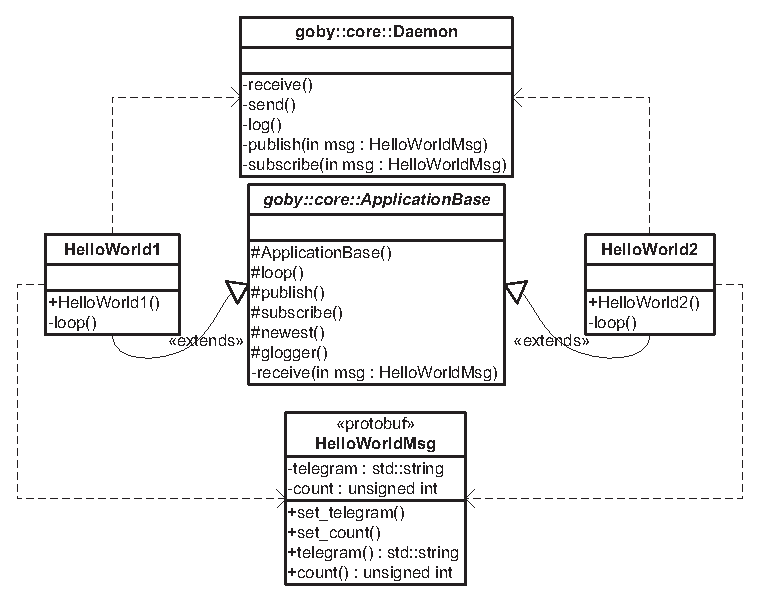
\includegraphics[scale=0.9]{hello_world_structure}
\caption{Structure diagram of the Hello World example showing the classes and dependencies. \texttt{HelloWorld1} and \texttt{HelloWorld2} are both Goby applications and thus are classes derived (solid arrows) from \texttt{goby::core::ApplicationBase}. Both of them (dashed arrows) depend on the Protocol Buffers message \texttt{HelloWorldMsg} because they use it to communicate. They also both depend on \texttt{goby::core::Daemon} (\texttt{gobyd}) for passing this message. See Fig. \ref{fig:hellow_world_sequence} for the sequence of sending a message in this example.}
\label{fig:hellow_world_structure}
\end{figure}

\section{Meeting goby::core::ApplicationBase}

\verb|goby::core::ApplicationBase| is the building block (base class\footnote{also called a superclass or parent class}) upon which we will make our Goby applications (which will be derived classes \footnote{also known as subclass or child class} of ApplicationBase). \verb|ApplicationBase| provides us with a number of tools; the main ones are:

\begin{itemize}
\item a constructor \textit{ApplicationBase()} that reads the command line and configuration (we will learn about this later) and connects to the Goby Daemon (\verb|gobyd|) for us.
\item a virtual method \textit{loop()} that is called at a regular frequency which is 10 Hertz by default. We will learn how to change the frequency at which \textit{loop()} is called later. 
\item a method \textit{subscribe()} which tells \verb|gobyd| that we wish to receive all messages of this type.
\item a method \textit{newest()} which returns the newest (latest received) message of a given type that we have previously called \textit{subscribe()} for. We will learn how to filter the subscriptions later.
\item a method \textit{publish()} allowing us to publish messages to \verb|gobyd| and thereby to any subscribers of that type.
\item a method \textit{glogger()} which acts just like std::cout\footnote{\textit{glogger()} accesses an instantiation of goby::util::FlexOstream, a derived class of std::ostream. std::cout is also a derived class of std::ostream.} and lets us write to the debug (terminal window / text file) \textit{g}oby \textit{logger}.
\end{itemize}


\begin{figure}
\centering
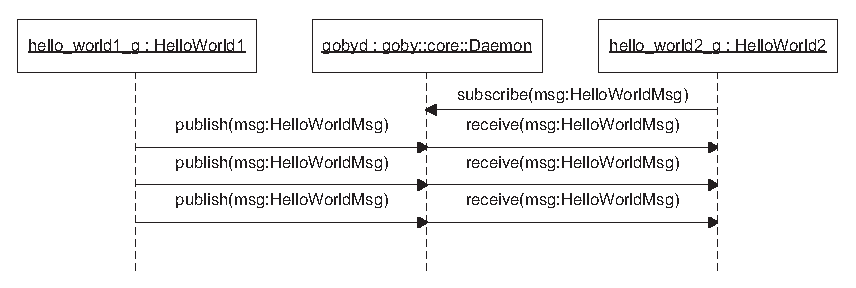
\includegraphics[scale=0.9]{hello_world_sequence}
\caption{Sequence diagram of the Hello World example. \texttt{HelloWorld2} subscribes for all messages of type \texttt{HelloWorldMsg} after which \texttt{HelloWorld1} publishes repeatedly a \texttt{HelloWorldMsg} that is processed and sent by \texttt{gobyd} to all subscribers (in this case just \texttt{HelloWorld2}).}
\label{fig:hellow_world_sequence}
\end{figure}


\section{Creating a simple Google Protocol Buffers Message: HelloWorldMsg}\label{sec:proto_ex}

Google Protocol Buffers\footnote{The Protocol Buffers project documented here: \url{http://code.google.com/apis/protocolbuffers/docs/overview.html}} (or protobuf for short) allows us to create custom objects for holding and transmitting data in a structured fashion. Transmitting data typically is done in a long string of bytes. However, humans do not view the world as a string of bytes. We think and communicate using tangible and intangible objects. For example, a baseball might be described by its diameter, color, weight, and materials. Goby (using protobuf objects) allows messages to be formed using this more natural representation.

The protobuf language is simple with a syntax similar to that of C. Protocol Buffers messages are written in .proto files and passed to the protobuf compiler (\verb|protoc|) which generates C++ code to pass to the C++ compiler (\verb|gcc| on Linux). Protobuf messages can contain a number of basic types (or vectors of these types) as well as nested messages. Fields are labeled as required, optional or repeated (essentially a vector). Required fields must be filled in; clearly, optional fields can be omitted. This might be a good time to read the \href{http://code.google.com/apis/protocolbuffers/docs/cpptutorial.html}{Protocol Buffers tutorial} to get a feel for the language and usage.

As you become familiar with using Protocol Buffers, the \href{http://code.google.com/apis/protocolbuffers/docs/proto.html}{language reference} will help you in creating .proto files and the \href{http://code.google.com/apis/protocolbuffers/docs/reference/cpp-generated.html}{generated code reference} will assist you in accessing the C++ classes created by the .proto files when passed through \verb|protoc|.

For this example, we wish to send ``hello world'' (of course) so we need a string to hold our message that we will call `telegram'. Furthermore, we want to keep track of how many times we've said ``hello'' so we'll add an unsigned integer called `count'. The resulting \href{http://bazaar.launchpad.net/~goby-dev/goby/trunk/annotate/head:/src/core/examples/ex1_hello_world/hello_world.proto}{.proto file} should now be clear:
\begin{boxedverbatim}
// protocol buffers language (similar to C)
message HelloWorldMsg
{
  required string telegram = 1;
  required uint32 count = 2;
}
\end{boxedverbatim}
\resetbvlinenumber
We chose ``required'' to prefix both fields because we feel that a valid \verb|HelloWorldMsg| must contain both a ``telegram'' and a ``count.'' \verb|uint32| is an unsigned (non-negative) 32 bit integer. The numbers following the ``='' sign are unique identifiers for each field. These numbers can be chosen however one likes as long as they are unique within a given protobuf message. Ascending numbers in the order fields are declared in the file is a reasonable choice.

This .proto file is ``compiled'' into a class with the same name as the message (\verb|HelloWorldMsg|). This class is accessed by including a header file with the same name as the .proto file, but with ``.proto'' replaced with ``.pb.h''. Furthermore, we can set the contents of this class using calls (``mutators'' or ``setters'') that are the same as the field name (i.e. ``telegram'' or ''count'') prepended with ``set\_'':
\begin{boxedverbatim}
// C++ 
#include "hello_world.pb.h"

// create and populate a ``HelloWorldMsg'' called `msg'
HelloWorldMsg msg;
msg.set_telegram("hello world");
msg.set_count(3);
\end{boxedverbatim}
\resetbvlinenumber

and access them using these methods (``accessors'' or ``getters'') that have the same function name as the field name:

\begin{boxedverbatim}
// C++ 
// print information about `msg' to the screen
std::cout << msg.telegram() << ": " << msg.count() << std::endl;
\end{boxedverbatim}
\resetbvlinenumber


\section{Learning how to \textit{publish}: HelloWorld1}

To create a Goby application, one needs to

\begin{itemize}
\item create a derived class of \verb|goby::core::ApplicationBase|. This is created by the following declaration:
\begin{boxedverbatim}
class HelloWorld1 : public goby::core::ApplicationBase {};
\end{boxedverbatim}
\resetbvlinenumber
We also must include the goby core header:
\begin{boxedverbatim}
#include "goby/core/core.h"
\end{boxedverbatim}
\resetbvlinenumber
\item run the application using the \textit{goby::run()} function. Because goby::core::ApplicationBase reads our configuration (including command line options) for us, we also pass argv and argc to \textit{run()}:
\begin{boxedverbatim}
int main(int argc, char* argv[])
{   
    return goby::run<HelloWorld1>(argc, argv);
}
\end{boxedverbatim}
\resetbvlinenumber
\end{itemize}
That is all one needs to create a valid working Goby application. All together the ``bare-bones'' Goby application looks like:

\begin{boxedverbatim}
#include "goby/core/core.h"

class HelloWorld1 : public goby::core::ApplicationBase {};

int main(int argc, char* argv[])
{   
    return goby::run<HelloWorld1>(argc, argv);
}
\end{boxedverbatim}
\resetbvlinenumber

However, we would like our application to do a little bit more.

ApplicationBase provides a \href{http://www.cplusplus.com/doc/tutorial/polymorphism/}{virtual method} called \textit{loop()} that is called on some regular interval (it is the \textit{synchronous event} in Goby), by default 10 Hertz. By overloading \textit{loop()} in our derived class \verb|HelloWorld1|, we can do any kind of synchronous work that needs to be done without tying up the CPU all the time\footnote{in between calls to \textit{loop()}, ApplicationBase handles incoming subscribed messages}. In this example, we will create a simple message (of type HelloWorldMsg which we previously designed in chapter \ref{sec:proto_ex}) and publish it to \verb|gobyd| and thus all subscribers (we create a subscriber in chapter \ref{sec:sub_ex}). 

Let's walk through each line of our \textit{loop()} method:

\begin{boxedverbatim}
void loop()
{
   static int i = 0;
   HelloWorldMsg msg;
   msg.set_telegram("hello world!");
   msg.set_count(++i);
   glogger() << "sending: " << msg << std::endl;
   publish(msg);
}
\end{boxedverbatim}
\resetbvlinenumber

Line 1: \textit{loop()} takes no arguments and returns nothing (void). We declare (line 3) a static integer\footnote{static in this context means that the variable will keep its value across calls to the function \textit{loop()}.} to keep track of how many times we have looped and thus print an increasing integer value. Then we create a HelloWorldMsg called msg (line 4) and set the values of its fields (lines 5 and 6). We then publish a human debugging log message using \textit{glogger()} (just like std::cout or other std::ostreams), which will be put to the terminal window in verbose mode\footnote{goby provides operator<< for google::protobuf::Message objects as a wrapper for google::protobuf::Message::DebugString()}. Finally, we publish our message (line 8).

\section{Learning how to \textit{subscribe}: HelloWorld2} \label{sec:sub_ex}

Now that our hello\_world1\_g application is publishing a message, we would like to create an application that subscribes for it. To subscribe for a message, we typically provide two things:
\begin{itemize}
\item The type of the message we want to subscribe for (e.g. HelloWorldMsg).
\item A method or function that should be called when we receive that type (a callback).
\end{itemize}

Subscriptions typically take place in the constructor (here, HelloWorld2::HelloWorld2()), but can happen at any time as needed (within \textit{loop()}, for example). You subscribe for a type once, and then you will continue to receive all other applications' publishes to that type.

We subscribe for a type using a call to \textit{subscribe()} that looks like this:
\begin{boxedverbatim}
subscribe<HelloWorldMsg>(&HelloWorld2::receive_msg, this);
\end{boxedverbatim}
\resetbvlinenumber

While a bit complicated at first, this call should make sense shortly. It reads ``\textit{subscribe} for all messages of type \textit{HelloWorldMsg} and when you receive one, call the method \textit{HelloWorld2::receive\_msg} which is a member of \textit{this} class (HelloWorld2).''\footnote{You can call a member function (method) of another class by passing the pointer to the desired class instantiation instead of \textit{this}. Alternatively, you can call a non-class function by just giving its pointer, e.g. subscribe(\&receive\_msg).}. The method provided as a callback (here \textit{receive\_msg()}) must have the signature
\begin{boxedverbatim}
void func(const ProtoBufMessage&); 
\end{boxedverbatim}
\resetbvlinenumber
where ProtoBufMessage is the type subscribed for (here, HelloWorldMsg). \textit{receive\_msg()} has that signature
\begin{boxedverbatim}
void HelloWorld2::receive_msg(const HelloWorldMsg& msg);
\end{boxedverbatim}
\resetbvlinenumber
and thus is a valid callback for this subscription. \textit{receive\_msg()} will be called immediately (an \textit{asynchronous} event) upon receipt of a message of type HelloWorldMsg unless
\begin{itemize}
\item \textit{loop()} is in the process of being called or
\item another message callback is in the process of being called.
\end{itemize}
In these cases, \textit{receive\_msg()} is called as soon as the blocking method returns. Inside of \textit{receive\_msg()} we simply post the message to the debug log:

\begin{boxedverbatim}
void receive_msg(const HelloWorldMsg& msg)
{
   glogger() << "received: " << msg << std::endl;
}
\end{boxedverbatim}
\resetbvlinenumber

\section{Compiling our applications using CMake}

\href{http://www.cmake.org/}{CMake}, while still lacking in documentation, is probably the easiest way to build software these days, especially for cross platform support. I will briefly walk through building a Goby application using CMake within the larger Goby project configuration. If you look at the \verb|CMakeLists.txt| file in \href{http://bazaar.launchpad.net/~goby-dev/goby/trunk/annotate/head:/src/core/examples/ex1_hello_world/CMakeLists.txt}{goby/src/core/examples/ex\_hello\_world/CMakeLists.txt}, you can see the steps needed to add our new applications to the project:

\begin{boxedverbatim}
protobuf_generate_cpp(PROTO_SRCS PROTO_HDRS hello_world.proto)
add_executable(hello_world1_g hello_world1.cpp ${PROTO_SRCS} ${PROTO_HDRS})
target_link_libraries(hello_world1_g goby_core)
\end{boxedverbatim}
\resetbvlinenumber

Line 1 tells CMake to add ``hello\_world.proto'' to the files needed to be pre-compiled by the Google Protocol Buffers compiler \verb|protoc|. protobuf\_generate\_cpp is provided by the CMake module \href{http://bazaar.launchpad.net/~goby-dev/goby/trunk/annotate/head:/cmake_modules/FindProtobufGoby.cmake}{goby/cmake\_modules/FindProtobufGoby.cmake}. Line 2 adds our application \verb|hello_world1_g| to the list to be compiled by the C++ compiler, using the sources \verb|hello_world1.cpp| and the generated Protocol Buffers code. We append ``\_g'' as a convention to quickly recognize Goby applications. Line 3 links our application against the goby\_core library, which provides goby::core::ApplicationBase, our base class.

Adding \verb|hello_world2_g| is directly analogous.

\section{Trying it all out: running from the command line}

Now, assuming you've \href{http://gobysoft.com/doc}{gone and compiled} everything, we can run the example.

You'll need three terminal windows, one for \verb|gobyd|, and one for each of our ``hello world'' applications. You need to start \verb|gobyd| first
\begin{boxedverbatim}
> gobyd -p hello_auv
\end{boxedverbatim}
\resetbvlinenumber
I've gone ahead and named this platform ``hello\_auv''. The platform name is a unique identifier for both intra- and inter-vehicle communications in Goby. Now we can launch our two applications (order doesn't matter), with the added ``-v'' flag to indicate we want verbose terminal output:

\begin{boxedverbatim}
> hello_world1_g -p hello_auv -v
> hello_world2_g -p hello_auv -v
\end{boxedverbatim}
\resetbvlinenumber

You should see \verb|hello_world1_g| passing messages to \verb|hello_world2_g| every 1/10th second.

\chapter{The GPS Driver example}

Marine robots need to know where they are. The simplest way now is to use a GPS receiver. While this works only when the robot is on the surface of the ocean, it is one of the most accurate forms of positioning available and thus used as a starting point for undersea dead reckoning using Doppler Velocity Loggers (DVLs) or Inertial Measurement Units (IMUs). Therefore, reading a GPS receiver's output into a usable form for decision making is a useful and necessary ability for our marine robot. This example shows how we might do this using Goby.

Typically we might also need to know the depth of our vehicle. This is often determined by measuring the ambient pressure. In this example, we will simulate the scalar depth reading of such a pressure sensor.

Finally, it is often useful to have an aggregate of the vehicle's status that includes a snapshot of the vehicle's location, orientation, speed, heading, and perhaps other factors such as battery life and health. For this example, we call such a message a ``NodeReport'' and provide an application ``node\_reporter\_g'' that compiles the reports from the GPS and the depth sensor into a single message. To extend this example, we could add data from other sources, such as an inertial measurement unit (IMU) or Doppler Velocity Logger (DVL).

As the first example, the files for this example are located in \href{http://bazaar.launchpad.net/~goby-dev/goby/trunk/files/head:/src/core/examples/ex2_gps_driver}{goby/src/core/examples/ex2\_gps\_driver} for your reference. 

\section{Reading \textit{configuration} from files and command line: DepthSimulator}

``DepthSimulator'' is reads a starting depth value from a configuration file and reports that value as the current depth, perturbed slightly by a random value. It's a primitive constant depth simulator, but allows us to illustrate another feature of Goby, the configuration file reader.

Goby reads configuration text files and the command line also using Google Protocol Buffers. The Goby application author provides a .proto file containing a protobuf message that defines the valid configuration for the given application. Then the application instantiates a copy of this configuration message and passes it to the \verb|goby::core::ApplicationBase| constructor with reads the configuration text file and/or command line options. If the configuration text file and/or command line options properly populate the provided proper configuration protobuf message, the message is returned to the derived class (the Goby application). Otherwise, execution of the application ends with a useful error message for the user explaining the errors involved with the passed configuration. 

Thus, for the ``DepthSimulator'' we define a protobuf message called DepthSimulatorConfig (in \href{http://bazaar.launchpad.net/~goby-dev/goby/trunk/annotate/head:/src/core/examples/ex2_gps_driver/config.proto}{goby/src/core/examples/ex2\_gps\_driver/config.proto}):

\begin{boxedverbatim}
message DepthSimulatorConfig
{
  required AppBaseConfig base = 1;
  required double depth = 2;
}
\end{boxedverbatim}
\resetbvlinenumber

An embedded message of type \verb|AppBaseConfig| is always provided for configuring parameters common for all Goby applications, such as the frequency that the virtual method \textit{loop()} is called, the name of the application to use with \verb|gobyd| (if different from the compiled name), and the name of the platform that this application belongs on (and thus which gobyd to connect to if multiple \verb|gobyd|s are running on a single computer). The AppBaseConfig message is defined in \href{http://bazaar.launchpad.net/~goby-dev/goby/trunk/annotate/head:/src/core/proto/app_base_config.proto}{goby/src/core/proto/app\_base\_config.proto}.

Specifically, for our DepthSimulator, we only have one other configuration parameter, a double called ``depth''. It is required, so our application will fail to run without a depth provided.

To use the Goby configuration reader, we create an instantation of our DepthSimulatorConfig
\begin{boxedverbatim}
class DepthSimulator : public goby::core::ApplicationBase
{ 
...
    static DepthSimulatorConfig cfg_;
};
\end{boxedverbatim}
\resetbvlinenumber
which must either be a global object or a static member of our class so that it is instantiated before the goby::core::ApplicationBase (normal members of our DepthSimulator class would be instantiated \textit{after} ApplicationBase, which would lead to trouble when ApplicationBase tried to use the object).

Then, all we must do is pass a pointer to that object to the constructor of the base class:
\begin{boxedverbatim}
    DepthSimulator()
        : goby::core::ApplicationBase(&cfg_)
\end{boxedverbatim}
\resetbvlinenumber
goby::core::ApplicationBase will take of the rest. To see what configuration values can be used in our compiled \verb|depth_simulator_g|, we can run it with the -h or --help flag:
\begin{boxedverbatim}
> depth_simulator_g --help
\end{boxedverbatim}
\resetbvlinenumber

which should provides output 
\begin{boxedverbatim}
Allowed options:

Typically given in depth_simulator_g configuration file,
but may be specified on the command line:
  --base arg             (req)
                          platform_name: "AUV-23"  same as self.name for 
                                                   gobyd cfg (req)
                          app_name: "myapp_g"  default is compiled name - 
                                               change this to run multiple 
                                               instances (opt)
                          verbosity: QUIET  Terminal verbosity 
                                            (opt) (default)
                          loop_freq: 10  the frequency (Hz) used to run 
                                         loop() (opt) (default)
  --depth arg            (req)

Given on command line only:
  -c [ --cfg_path ] arg      path to depth_simulator_g configuration file 
                             (typically depth_simulator_g.cfg)
  -h [ --help ]              writes this help message
  -p [ --platform_name ] arg name of this platform (same as gobyd configuration
                             value `self.name`)
  -a [ --app_name ] arg      name to use when connecting to gobyd (default: 
                             depth_simulator_g)
  -v [ --verbose ] arg       output useful information to std::cout. -v is 
                             verbosity: verbose, -vv is verbosity: debug, -vvv 
                             is verbosity: gui
\end{boxedverbatim}
\resetbvlinenumber

Thus, to configure \verb|depth_simulator_g| I could create a text file (let's say depth\_simulator.cfg) with values like
\begin{boxedverbatim}
# depth_simulator.cfg
base
{
    platform_name: "AUV-1"
    loop_freq: 1
}

depth: 10.4
\end{boxedverbatim}
\resetbvlinenumber

Then, when we run \verb|depth_simulator_g| we pass the path to the configuration file as the first command line option:
\begin{boxedverbatim}
> depth_simulator_g depth_simulator.cfg 
\end{boxedverbatim}
\resetbvlinenumber

If we didn't want to use a configuration file, we could pass the same contents of the depth\_simulator.cfg file given above on the command line instead:
\begin{boxedverbatim}
> depth_simulator_g --base 'platform_name: "AUV-1" loop_freq: 1' --depth 10.4
\end{boxedverbatim}
\resetbvlinenumber

If the same configuration values are provided in both the configuration file and on the command line, they are merged for ``repeat'' fields. For ``required'' or ``optional'' fields, the command line value overwrites the configuration file value. 

Thus, if we run
\begin{boxedverbatim}
> depth_simulator_g depth_simulator.cfg --depth 20.5
\end{boxedverbatim}
\resetbvlinenumber
\verb|cfg_.depth()| is 20.5 since the command line provided value takes precedence.

Some commonly used configuration values have shortcuts for the command line. For example, the following two commands are equivalent ways to set the platform name:
\begin{boxedverbatim}
> depth_simulator_g --base 'platform_name: "AUV-1"'
> depth_simulator_g -p "AUV-1"
\end{boxedverbatim}
\resetbvlinenumber

Other than reading a configuration file, all ``DepthSimulator'' does is repeatedly write a message of type DepthReading (see \href{http://bazaar.launchpad.net/~goby-dev/goby/trunk/annotate/head:/src/core/examples/ex2_gps_driver/depth_reading.proto}{goby/src/core/examples/ex2\_gps\_driver/depth\_reading.proto}) based off a random offset to the configuration value ``depth'':
\begin{boxedverbatim}
void loop()
    {
       DepthReading reading;
       // just post the depth given in the configuration file plus a small random offset
       reading.set_depth(cfg_.depth() + (rand() % 10) / 10.0);

       glogger() << reading << std::flush;
       publish(reading);    
    }
\end{boxedverbatim}
\resetbvlinenumber

You will note that depth\_reading.proto contains an import command and a field of type ``Header'':
\begin{boxedverbatim}
import "goby/core/proto/header.proto";

message DepthReading
{
  // time is in header
  required Header header = 1;
  required double depth = 2;
}
\end{boxedverbatim}
\resetbvlinenumber

``Header'' (defined in \href{http://bazaar.launchpad.net/~goby-dev/goby/trunk/annotate/head:/src/core/proto/header.proto}{goby/src/core/proto/header.proto}) provides commonly used fields such as time and source / destination addressing. It is highly recommended to include this in messages sent through Goby, but not required. goby::core::ApplicationBase will populate any required fields in ``Header'' not given by DepthSimulator. For example, if neither time field (unix\_time nor iso\_time) is set, goby::core::ApplicationBase will set the time based on the publish time. However either unix\_time or iso\_time should be set if the calling application has a better time stamp for the message than the publish time.

\section{Our first ``useful'' application: GPSDriver}

GPSDriver doesn't introduce any new features of Goby, but it attempts to be the first non-trivial application we have seen thus far. GPSDriver connects to a NMEA-0183 compatible GPS receiver over a serial port, reads all the messages and parses the GGA sentence into a useful protobuf message for posting to the database (via \verb|gobyd|). 

\subsection{Configuration}
The configuration needed for GPSDriver all pertains to how the serial GPS receiver is connected and how it communicates:
\begin{boxedverbatim}
message GPSDriverConfig
{
  required AppBaseConfig base = 1;

  required string serial_port = 2;
  optional uint32 serial_baud = 3 [default = 4800];
  optional string end_line = 4 [default = "\r\n"];
}
\end{boxedverbatim}
\resetbvlinenumber

Note the use of defaults when they are meaningful (the NMEA-0183 specification requires carriage return and new line as the end line so this default will likely often be precisely what our users want, saving them the effort of specifying it every time).

\subsection{Protobuf Messages}
GPSDriver uses two protobuf messages both defined in \\ \href{http://bazaar.launchpad.net/~goby-dev/goby/trunk/annotate/head:/src/core/examples/ex2_gps_driver/gps_nmea.proto}{goby/src/core/examples/ex2\_gps\_driver/gps\_nmea.proto}. The first (NMEASentence) is a parsed version of a generic NMEA-0183 message. The second (GPSSentenceGGA) contains a NMEASentence but also parsed fields of the GGA position message. Providing the GPSSentenceGGA gives all subscribers of this message rapid access to useful data without parsing the original NMEA string again.

\subsection{Body}
GPSDriver should be straightforward to understand given what we have learned to this point. It makes use of some utilities in the goby::util libraries, especially the goby::util::SerialClient used for reading the serial port. These utilities are documented along with all the other Goby classes at \url{http://gobysoft.com/doc}.

Goby makes heavy use of the Boost libraries (\url{http://www.boost.org}). While you are not required to use any of Boost when developing Goby applications, it would be worth your while becoming acquainted with them. For example, the Boost Date-Time library gives a handy object oriented way to handle dates and times that far exceeds the abilities of ctime (time.h).

\section{Subscribing for \textit{multiple types}: NodeReporter}

NodeReporter subscribes to both the output of DepthSimulator (DepthReading) and GPSDriver (GPSSentenceGGA). Whenever either is published, a new NodeReport message is created as the aggregate of pieces of both messages. The NodeReport (defined in \\ \href{http://bazaar.launchpad.net/~goby-dev/goby/trunk/annotate/head:/src/core/xamples/ex2_gps_driver/node_report.proto}{goby/src/core/examples/ex2\_gps\_driver/node\_report.proto}) is a useful summation of the status of a given node (synonomously, platform). Because DepthReading and GPSSentenceGGA are published asynchronously, we also keep track of the delays between different parts of the NodeReport message (the *\_lag fields). 

The NodeReport provides
\begin{enumerate}
\item Name of the platform
\item Type of the platform (e.g. AUV, buoy)
\item The global position of the vehicle in geodetic coordinates (latitude, longitude, depth)
\item The local position of the vehicle in a local cartesian coordinate system (x, y, z) based off the datum defined in the configuration for \verb|gobyd|. This is generally more useful for vehicle operators than the global fix.
\item The Euler angles of the current vehicle pose: roll, pitch, yaw (heading). 
\item The speed of the vehicle.
\end{enumerate}

In this example, we only set the first three fields given above. The others would require further sensing capability than we have in this example.

\section{Putting it all together}

\appendix

\chapter{Goby MOOS Modules}

The acoustic communications portion of Goby was developed originally for the MOOS autonomy architecture. Thus, the relevant MOOS modules \verb|pAcommsHandler| and others are still maintained (in goby/src/moos) for the use of the MOOS-IvP community. MOOS-IvP is explained in \cite{moos-ivp-jfr} and is available at \url{http://moos-ivp.org}. The usage of these modules is documented here. See \url{http://gobysoft.com/doc/#install} for how to install Goby.

The beginning of this appendix motivates the current design, followed by a user manual for the individual MOOS processes.

\section{Unified Command and Control for Subsea Autonomous Sensing Networks}

The process of undersea observation, mapping, and monitoring is experiencing a dramatic
paradigm shift away from platform-centric, human-controlled sensing,
processing and interpretation. Rather, distributed sensing
using networks of autonomous platforms is becoming the preferred technique.
An optimal platform suite is often highly heterogeneous with large differences in mobility,
maneuverability, sensing capability, and communication connectivity.  The
sensor systems have different constraints on platform mobility and
communication capacity, and some network operations require highly
coordinated maneuvering of heterogeneous platforms. Unified Command and Control \cite{unified_c2} is a new command and control paradigm inherently suited for such heterogeneous networks. Implemented using
\verb|MOOS-IvP|, Nested Autonomy provides the fully integrated sensing,
modeling and control that allows each platform, on its own or in
collaboration with partners of opportunity, to autonomously detect,
classify, localize and track (DCLT) an episodic, natural or human-created event, and
subsequently report back to the operators.

A robust undersea communication infrastructure is crucial to the
operation of such networks. In contrast to air and land-based
equivalents, the extremely limited bandwidth, latency and
intermittency of underwater acoustic communication imposes severe
requirements to the selectivity of message handling. Thus, contact and
track reports for high-priority event, such as a detected chemical
plume from a deep ocean vent,  which may indicate an imminent volcanic
eruption, must be transmitted to the system operators without delay. On the
other hand, reports concerning less important events and platform status 
reports may be delayed without significant effects.
Previous message handling systems for underwater communications have only a
rigid, hard-coded queuing infrastructure, and do not support such
advanced priority-based selectivity, hampering the type and
amount of information that can be passed between cooperating nodes in
the network. This severely limits the level of autonomy that can be
supported on the network nodes.

\begin{figure}[tp]
  \centering 
  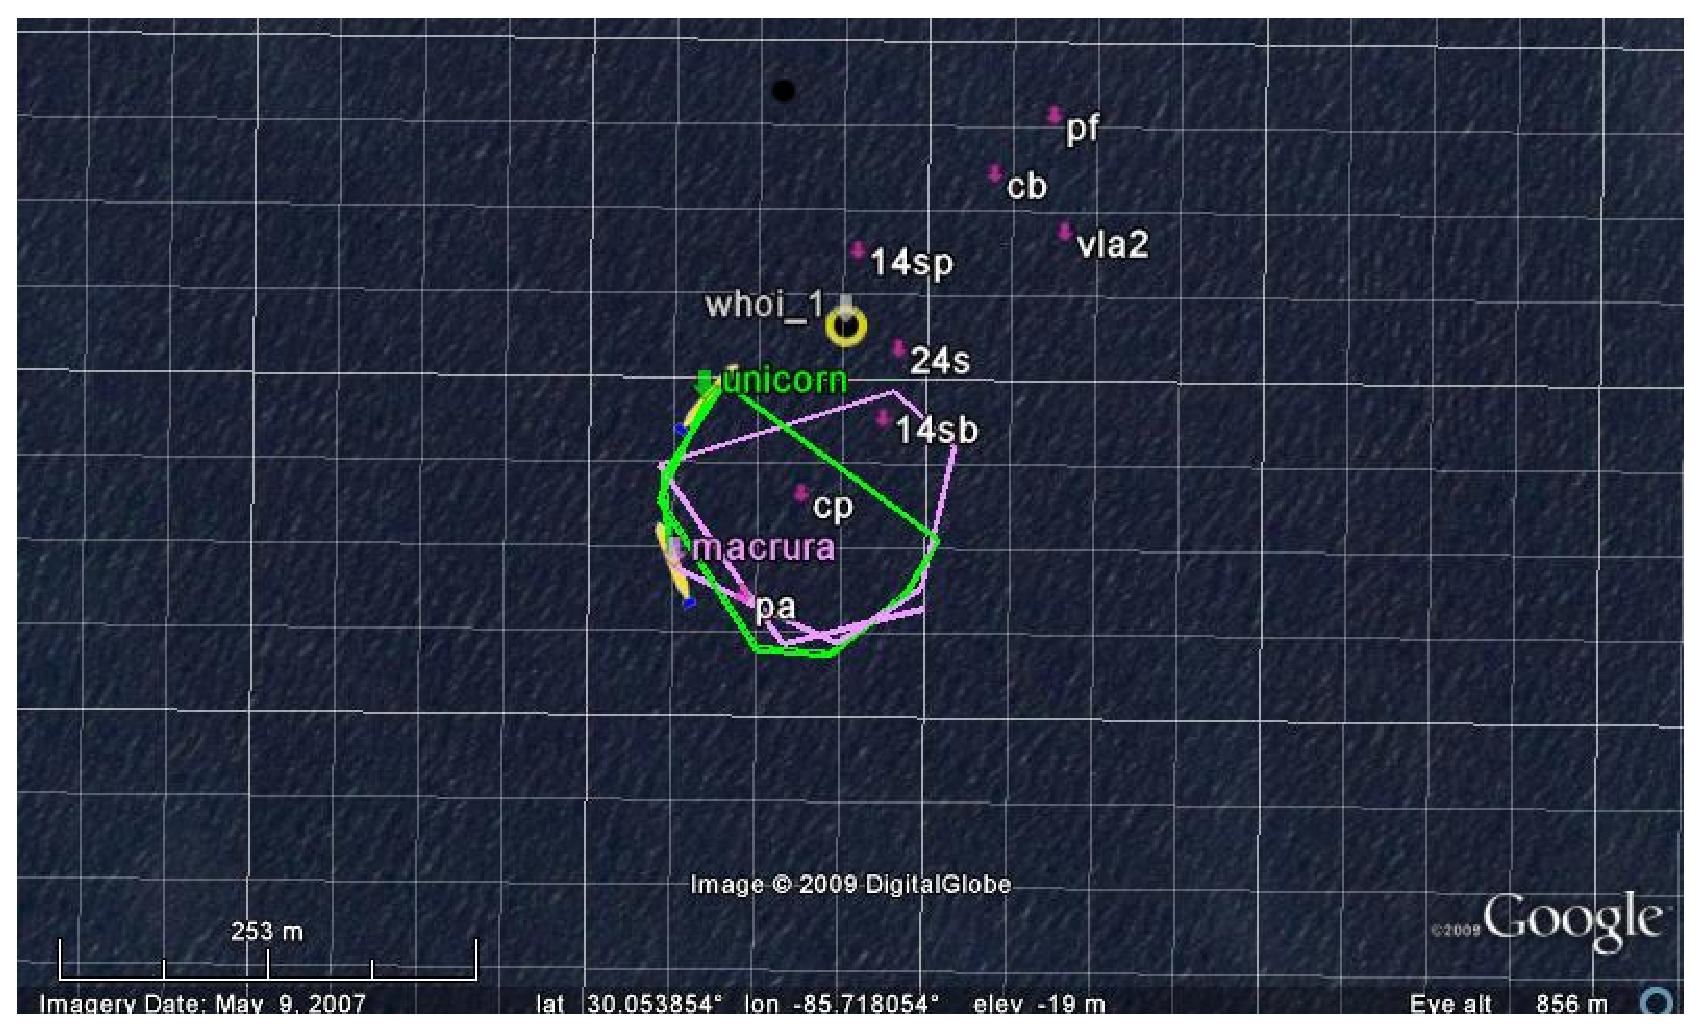
\includegraphics[width=0.75\textwidth]{bistatic3.eps}
\caption{ Collaborative autonomy demonstrated in SWAMSI09 using MIT
  LAMSS communication stack. The two BF21 AUVs Unicorn and Macrura
  perform synchronized swimming maintaining a constant bistatic angle
  of $60^{\circ}$ relative to a proud cylindrical target
  (cp). \label{bistatic3}}
\end{figure}

In response to this problem, a new MOOS-IvP communication software stack was developed at
the MIT Laboratory for Autonomous Marine Sensing Systems (LAMSS), in
support of autonomous sensing programs such as the ONR ASAP MURI,
GOATS, and SWAMSI. This new stack has enabled the operation of a communication
infrastructure which provides robust message handling for
collaborative autonomous sensing by heterogeneous, undersea autonomous
assets, as demonstrated in a handful of major recent field
experiments. As an example, Fig.~\ref{bistatic3} shows the
collaborative, multistatic MCM mission by the Unicorn and Macrura BF21
AUVs during SWAMSI09 in Panama City, FL. The two vehicles are circling
a proud cylinder (cp) at a distance of 80 m maintaining a constant
bistatic angle of 60 degrees. The collaboration was achieved fully
autonomously without any intervention by the operators, with each
vehicle adapting its speed based on its current position and the
position of the other vehicle extrapolated from the latest status,
contact or track report. Such collaborative maneuvers would not be
possible using traditional communication schemes, where navigation
packets must be rigidly interleaved with messages containg data and
command and control sequences. In contrast, the Dynamic Compact
Control Language (DCCL) used by the LAMSS communication
stack allows for adequate navigation information to be packed with all
other required message content.

Being based on established libraries of message handling software, the
open source architecture of this new MOOS communication stack lends
itself directly to a wide range of military and civilian
applications. It supports an arbitrary message suite and
content without requirement of modifying software. All message encoding and
decoding information is specified in a mission-unique configuration
file written in the standard XML format. Not only does this ensure
maximal flexibility in regard to message design, but it inherently
enables arbitrary levels of encryption for LPI/LPD communication
networks.

\section{Overview of the LAMSS Communication Stack}

\begin{figure}[tp]
  \centering 
  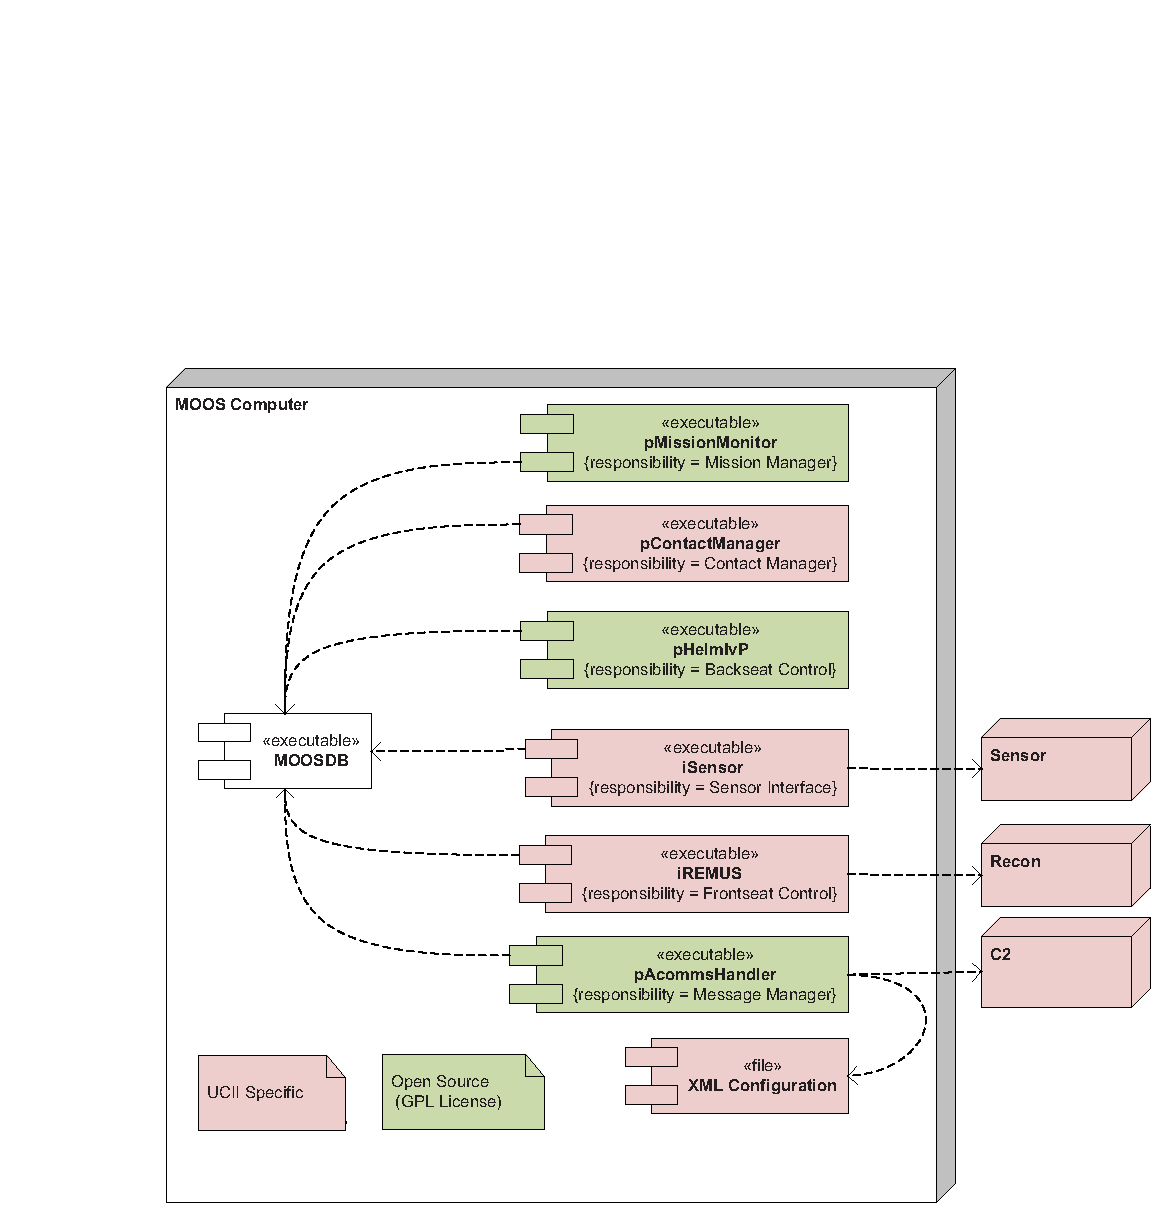
\includegraphics[width=\textwidth]{dclt_component.eps}
\caption{Incorporation of the open source LAMSS communication stack into
 a MOOS-IvP DCLT Autonomy System. The green boxes identify the
 open source modules, including the IvP Helm, the generic mission
 manager module, and the communication stack. The red modules are
 project specific, including the frontseat driver module, and the
 sensor modules. Also the message configuration specifying the message
 content and the coding, is project specific. \label{lamss_dclt}} 
\end{figure}

MIT LAMSS has over the last decade focused its research on the
development of sensor-adaptive, collaborative, autonomous sensing
concepts for the capture of episodic undersea events, including the
mapping of coastal fronts, chemical plumes, and natural and man-made
underwater acoustic sources. All these applications involve the
Detection, Classification, Localization and Tracking (DCLT) of the
event. To exploit the benefits of having multiple platforms involved
in tracking the event, an underwater robust communication system is
obviously a requirement. On the other hand, the communication capacity
of such systems is many orders of magnitude below land- and air-based
equivalents, requiring a much higher level of data compression and
on-board processing and decision-making than is required in air-based
systems. {\em Nested Autonomy}, developed over the
last decade by LAMSS, is an example of such an autonomy-driven
undersea sensing concept. Although this concept is based on the
philosophy that the system must be able to achieve its mission
objective even during periods with no or limited communication, there
is obviously still a need for occasional communication, e.g. for
reporting detected events of interest.

The new MOOS-IvP communication stack alleviates some of the problems and limitations of the
existing software stacks in this regard. These software stacks in general were designed to
sequentially transmit all messages generated by the autonomy system,
with only a rigid, hard-coded priority-based message queuing
infrastructure.

In undersea autonomous systems the priorities of information generated
by the on-board processing are highly dynamic, depending on the
tactical situation and the criticality of the generated
information. Thus, for example, a contact report for a target of
interest obviously must bypass queued contact reports for less
significant targets. Also, in high-clutter environments, the number of
contact reports may by far exceed the communication capacity and on-board
priority-based filtering is required.

\begin{figure}[htp]
\centering 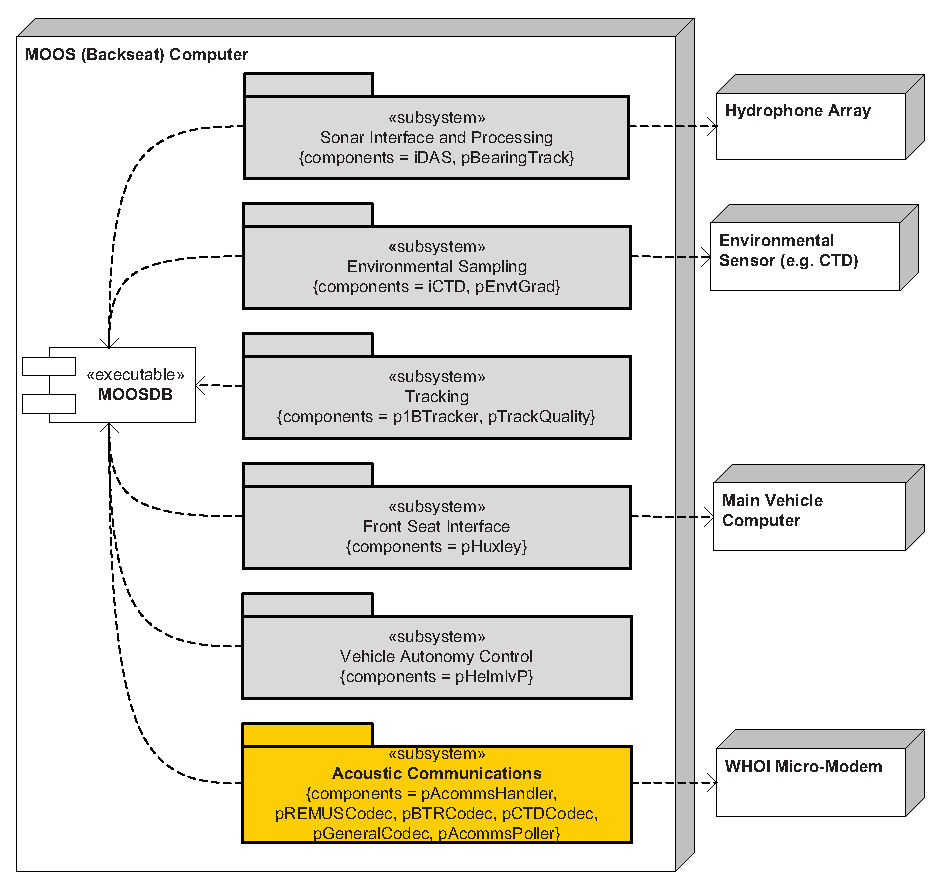
\includegraphics[width=\linewidth]{auv_community.eps}
\caption{MOOS-IvP community for MIT sonar AUVs, with the autonomous
  communication, command and control modules highlighted in
  gold. }
\label{fig:moos_comms}
\end{figure}

The incorporation of the MIT LAMSS communication stack into a MOOS-IvP
DCLT Autonomy System is illustrated in Fig.~\ref{lamss_dclt}. The
green boxes identify the Open Source modules, including the helm \verb|pHelmIvP|, the generic mission manager module \verb|pMissionMonitor|,
and the communication stack. The red modules are project-specific,
including the frontseat driver module \verb|iRemus|, the sensor
modules, and the contact manager process \verb|pContactManager|. Also
the message configuration files specifying the message content and the
coding specifics, are project-specific and not hard-wired into the
communication stack.

Figure \ref{fig:moos_comms} shows the communications subsystem as part of the whole
MIT LAMSS AUV MOOS community.




 Figure \ref{acomms_sequence} shows the sequence of commands for a single operator command message sent using iCommander.
 
 
\begin{figure}[tp]
  \centering 
  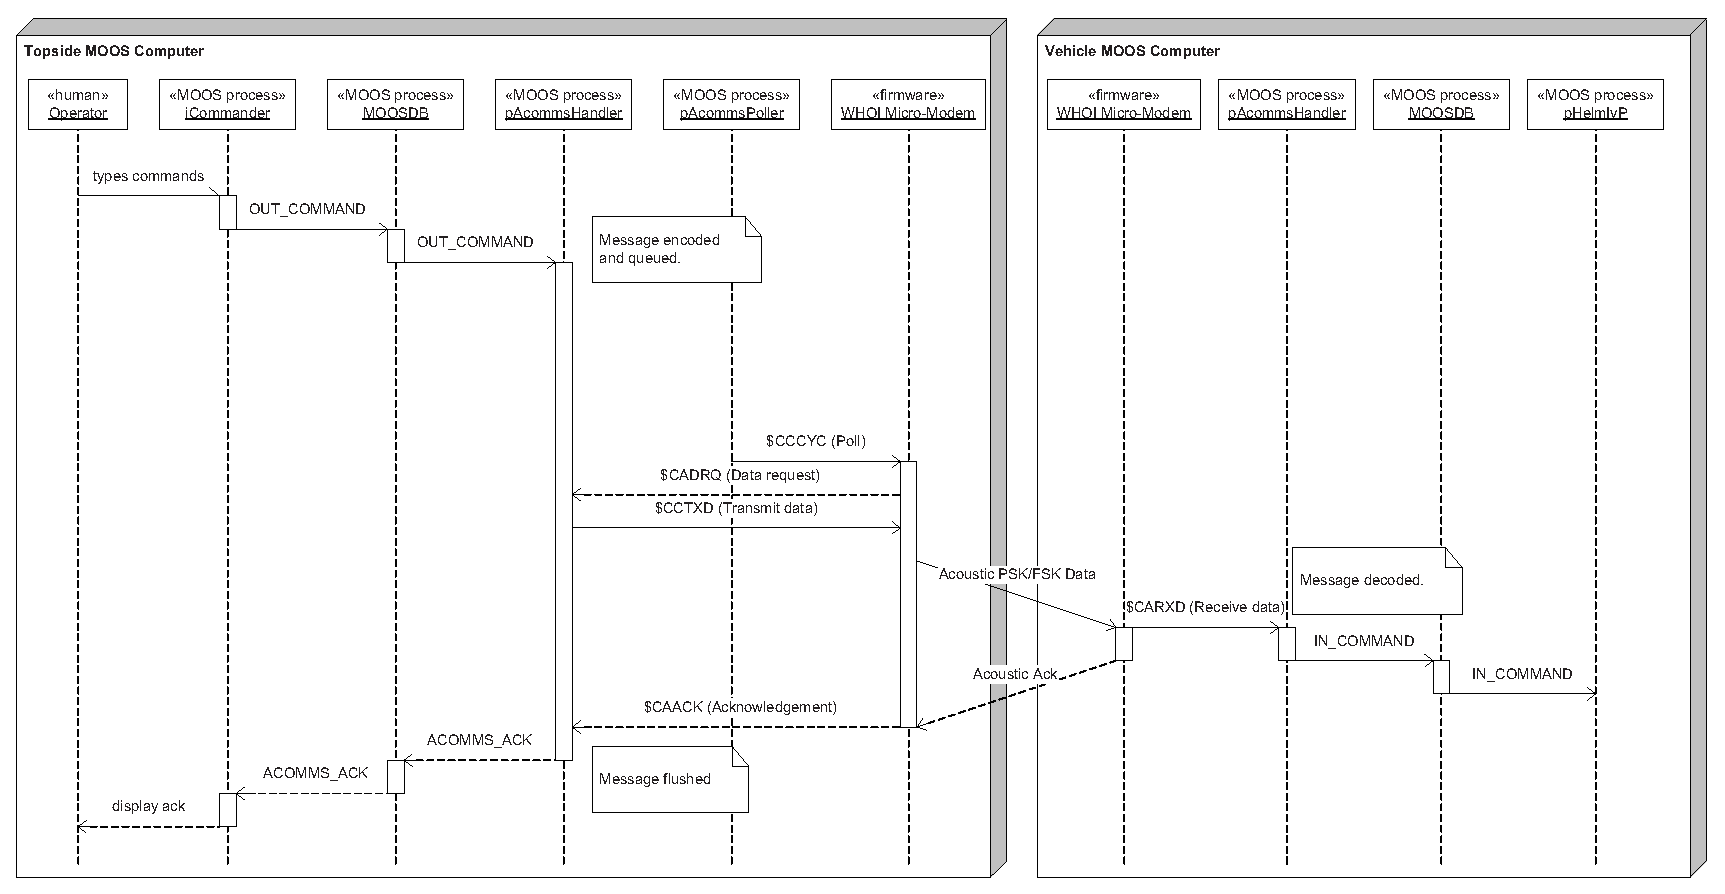
\includegraphics[width=1\textwidth]{acomms_sequence.eps}
\caption{UML Sequence diagram for sending a command to an AUV via the LAMSS Acoustic Communications Modules. \label{acomms_sequence}}
\end{figure}


The structure of the MIT LAMSS communication stack
is illustrated in Fig.~\ref{lamss_comms}.

\begin{figure}[tp]
  \centering 
  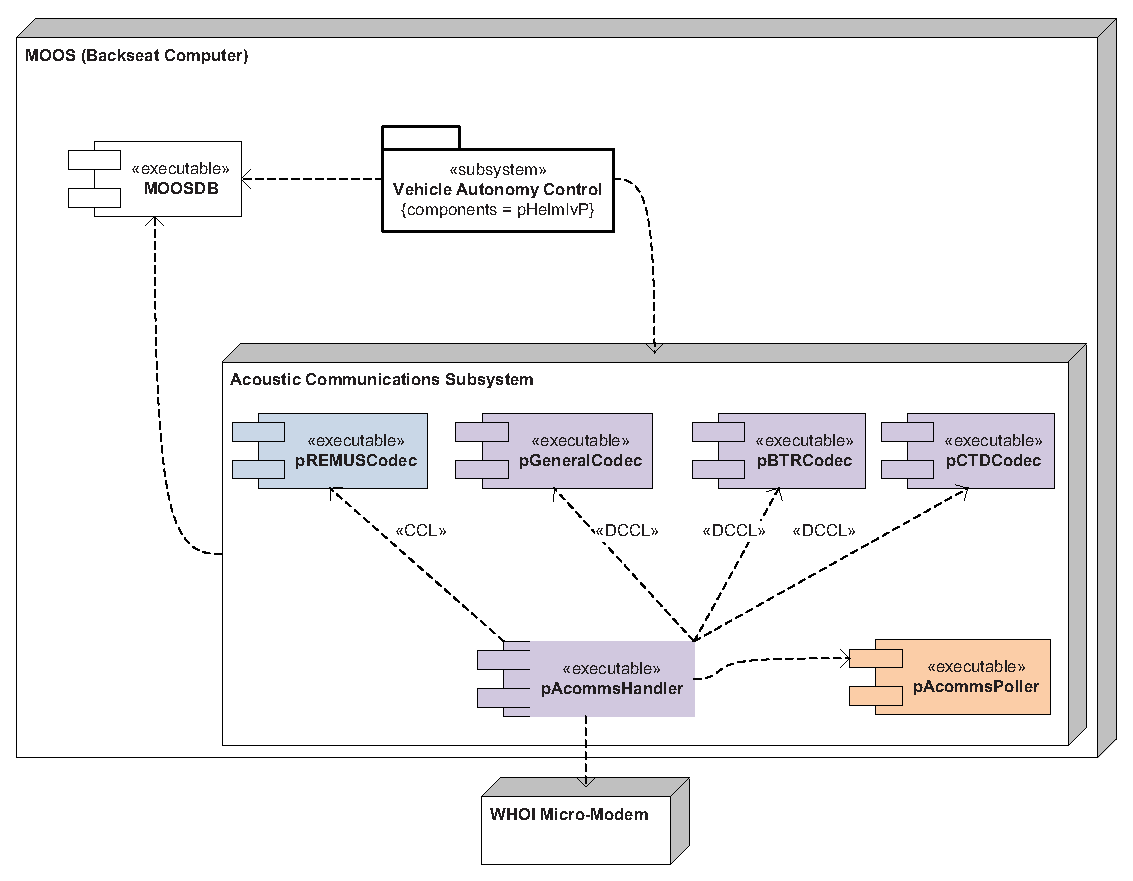
\includegraphics[width=\textwidth]{acomms_component.eps}
  \caption{UML Component Model of the MIT LAMSS communication stack. The principal
  message handler module is \texttt{pAcommsHandler}, which communicates
  directly with the modem using built-in drivers, and thus not
  dependent on third-party MOOS modem drivers. It also manages the
  message stream by a dynamic, priority-based queuing system. The
  message coding and decoding is performed by \texttt{pGeneralCodec} based on
  the rules set out in the configuration file, and dedicated DCCL
  codecs for transmitting various data streams.The stack also
  supports standard fixed Compact Control Language (CCL) messages such
  as the State message used by the Remus AUV, using dedicated codecs. Dashed line indicate dependencies between components. \label{lamss_comms}}
\end{figure}

\section{pAcommsHandler}
\label{sec:pacommshandler} 


\subsection{Problem}
Acoustic communications (in our case, with the WHOI Micro-Modem) are highly limited in throughput. Thus, it is unreasonable to expect ``total throughput'' of all communications data. Furthermore, even if total throughput is achievable over time, certain messages have a lower tolerance for delay (e.g. vehicle status) than others (e.g. CTD sample data). Reference  \url{http://acomms.whoi.edu/umodem/documentation.html} for more information on the WHOI Micro-Modem.

Also, in order to make the best use of this available bandwidth, messages need to be compacted to a minimal size before sending (effective encoding). To do this, pAcommsHandler provides an interface to the Dynamic Compact Control Language (DCCL\footnote{the name comes from the original CCL written by Roger Stokey for the REMUS AUVs, but with the ability to dynamically reconfigure messages based on mission need. DCCL is backwards compatible with a CCL network as it uses CCL message number 32}.) encoder/decoder. Furthermore, DCCL has powerful parsing abilities (``algorithms'') for both encoding and decoding, including the ability to perform certain geodesic conversions (e.g. latitude, longitude $\leftrightarrow$ UTM x,y) and lookups (e.g. \textit{modem\_id} $\leftrightarrow$ vehicle name) on data.

pAcommsHandler roughly performs the same functions of pFramer, pRouter, pAcommsPoller, and iMicroModem but
generalized to handle any number of message queues and extended to give more control over queue parameters. The DCCL encoding is much more flexible and more compact than the CCL encoding used by these older processes.

\subsection{Solution}
pAcommsHandler provides a(n):
\begin{enumerate}
\item Encoder/decoder unit (codec): encodes and decodes messages using DCCL (goby-acomms \verb|dccl| library), which reduces the data required to be sent by:
\begin{itemize}
\item Predefined messages: the user must specify a message structure what specifies what fields the message contains and how large each field should be (in an intuitive fashion that DCCL turns into bits). Both the sender and receiver have preshared knowledge of the message structure. From this knowledge, no meta information about the message (beyond an identifier) needs to be sent, simply the data. 
\item Custom field sizes: message fields are defined with custom tolerances (ranges and precisions) that are tighter than those given by the IEEE standards for floating point and integer numbers. For example, if a field needs to hold an integer that will never range outside [0, 1000] that field in the message will only be 10 bits long (ceil($\log_2{1001}$)).
\end{itemize}
\item Priority Queuing System: maintains an arbitrary number of message queues (each tied to a different MOOS variable) for hexadecimal data strings. (goby-acomms \verb|queue| library)
\begin{itemize} 
\item allows configuration of the queue priorities and dynamic growth of the priority over the time since the last sent message.
\item allows management of WHOI CCL message types as well as DCCL queuing. 
\end{itemize}
\item Modem Driver: handles all Micro-Modem serial communications. The driver (goby-acomms \verb|modemdriver| library) can be used with other modems besides the WHOI Micro-Modem (see \url{http://gobysoft.com/doc/acomms__driver.html#acomms_writedriver} for information on writing a new driver). 
\item MAC Manager: provides medium access control in the form of a simple slotted time division-multiple access (TDMA) scheme or flexible centralized polling.
\end{enumerate}

\subsection{Limitations}
pAcommsHandler \textit{does not}:

\begin{itemize}
\item provide any multi-hop routing. The sender and receiver must be directly in acoustic communications.
\item split user messages into packets. The user must provide data that are small enough to fit into the modem frame desired (32 - 256 bytes for the WHOI Micro-Modem).
\end{itemize} 

\subsection{Usage}
\subsubsection{Compilation}
pAcommsHandler depends on the Goby and MOOS libraries. See goby/DEPENDENCIES for help resolving the dependencies on your system.

\subsubsection{Parameters for the pAcommsHandler Configuration Block}\label{sec:pAcommsHandler:config}

\paragraph{Example moos file}

You can always get a complete listing of MOOS file parameters with their syntax by running
\begin{verbatim}
> pAcommsHandler --example_config
\end{verbatim}
\resetbvlinenumber

This is a complete list of all the configuration values pAcommsHandler accepts. Most of the time you will need far fewer configuration options to use it.

\begin{boxedverbatim}
ProcessConfig = pAcommsHandler
{
  common {  # Configuration common to all Goby MOOS applications 
            # (opt)
    log: true  # Should we write a text log of the terminal 
               # output? (opt) (default=true) (can also set MOOS 
               # global "log=")
    log_path: "./"  # Directory path to write the text log of the 
                    # terminal output (if log=true) (opt) 
                    # (default="./") (can also set MOOS global 
                    # "log_path=")
    community: "AUV23"  # The vehicle's name (opt) (can also set 
                        # MOOS global "Community=")
    lat_origin: 42.5  # Latitude in decimal degrees of the local 
                      # cartesian datum (opt) (can also set MOOS 
                      # global "LatOrigin=")
    lon_origin: 10.9  # Longitude in decimal degrees of the local 
                      # cartesian datum (opt) (can also set MOOS 
                      # global "LongOrigin=")
    app_tick: 10  # Frequency at which to run Iterate(). (opt) 
                  # (default=10)
    comm_tick: 10  # Frequency at which to call into the MOOSDB 
                   # for mail. (opt) (default=10)
    verbosity: VERBOSITY_VERBOSE  # Verbosity of the terminal 
                                  # window output (VERBOSITY_QUIET, 
                                  # VERBOSITY_WARN, 
                                  # VERBOSITY_VERBOSE, 
                                  # VERBOSITY_DEBUG, VERBOSITY_GUI) 
                                  # (opt) 
                                  # (default=VERBOSITY_VERBOSE)
    initializer {  # Publish a constant value to the MOOSDB at 
                   # startup (repeat)
      type: INI_DOUBLE  # type of MOOS variable to publish 
                        # (INI_DOUBLE, INI_STRING) (req)
      moos_var: "SOME_MOOS_VAR"  # name of MOOS variable to 
                                 # publish to (req)
      global_cfg_var: "LatOrigin"  # Optionally, instead of 
                                   # giving `sval` or `dval`, give 
                                   # a name here of a global MOOS 
                                   # variable (one at the top of 
                                   # the file) whose contents 
                                   # should be written to 
                                   # `moos_var` (opt)
      dval: 3.454  # Value to write for type==INI_DOUBLE (opt)
      sval: "a string"  # Value to write for type==INI_STRING 
                        # (opt)
    }
  }
  modem_id: 1  # Unique number 1-31 to identify this node (req)
  driver_type: DRIVER_NONE  # Corresponding driver for the type 
                            # of physical acoustic modem used 
                            # (DRIVER_NONE, DRIVER_WHOI_MICROMODEM, 
                            # DRIVER_ABC_EXAMPLE_MODEM) (opt) 
                            # (default=DRIVER_NONE)
  driver_cfg {  # Configure the acoustic modem driver (opt)
    modem_id: 1  # Unique number 1-31 to identify this node (req)
    connection_type: CONNECTION_SERIAL  # Physical connection 
                                        # type from this computer 
                                        # (running Goby) to the 
                                        # acoustic modem 
                                        # (CONNECTION_SERIAL, 
                                        # CONNECTION_TCP_AS_CLIENT, 
                                        # CONNECTION_TCP_AS_SERVER, 
                                        # CONNECTION_DUAL_UDP_BROADC
                                        # AST) (opt) 
                                        # (default=CONNECTION_SERIAL
                                        # )
    line_delimiter: "\r\n"  # String used to delimit new lines 
                            # for this acoustic modem (opt) 
                            # (default="\r\n")
    serial_port: "/dev/ttyS0"  # Serial port for 
                               # CONNECTION_SERIAL (opt)
    serial_baud: 19200  # Baud rate for CONNECTION_SERIAL (opt)
    tcp_server: "192.168.1.111"  # IP Address or domain name for 
                                 # the server if 
                                 # CONNECTION_TCP_AS_CLIENT (opt)
    tcp_port: 50010  # Port to serve on (for 
                     # CONNECTION_TCP_AS_SERVER) or to connect to 
                     # (for CONNECTION_TCP_AS_CLIENT) (opt)
          
    # extensions for the WHOI Micro-Modem Driver
    [MicroModemConfig.nvram_cfg]: "DTO,1" # send $CACFG,DTO,1 at launch
    [MicroModemConfig.reset_nvram]: true # reset NVRAM parameters to
                                         # factory defaults before
                                         # sending nvram_cfg values
    [MicroModemConfig.hydroid_gateway_id]: 1  # set to a non-zero value
        # to indicate that we are using the HYDROID gateway
        # buoy which has a non-standard sentence structure (#M / !M prefixes)
        # Omit for the normal WHOI Micro-Modem!
  }
  mac_cfg {  # Configure the acoustic Medium Access Control (opt)
    modem_id: 1  # Unique number 1-31 to identify this node (req)
    type: MAC_NONE  # The type of TDMA MAC scheme to use 
                    # (MAC_NONE, MAC_FIXED_DECENTRALIZED, 
                    # MAC_AUTO_DECENTRALIZED, MAC_POLLED) (opt) 
                    # (default=MAC_NONE)
    slot {  # Configure a slot in the communications cycle. Slots 
            # are run in the order they are declared. Omit for 
            # MAC_AUTO_DECENTRALIZED. (repeat)
      src: 1  # source modem id for this transmission (initiating 
              # platform) (req)
      dest: 0  # destination modem id for this transmission; 0 
               # means broadcast, -1 means query the queuing layer 
               # for next available message (opt) (default=0)
      rate: 0  # bit rate (integer from 0-5, 0 is slowest) (opt) 
               # (default=0)
      type: SLOT_DATA  # type of message to initiate in this slot 
                       # (SLOT_DATA, SLOT_PING, SLOT_REMUS_LBL) 
                       # (req) (default=SLOT_DATA)
      slot_seconds: 15  # length of this slot in seconds (opt)
      last_heard_time: ""  # used internally, no need to 
                           # configure manually (opt)
    }
    rate: 0  # Set rate to use for MAC_AUTO_DECENTALIZED. Use 
             # `slot` for other MACTypes (opt) (default=0)
    slot_seconds: 15  # Set duration of the slot for 
                      # MAC_AUTO_DECENTRALIZED. Use `slot` for 
                      # other MACTypes (opt) (default=15)
    expire_cycles: 30  # Set number of quiet cycles for 
                       # discarding a node from the cycle for 
                       # MAC_AUTO_DECENTRALIZED. (opt) (default=30)
  }
  queue_cfg {  # Configure the Priority Queuing layer (opt)
    modem_id: 1  # Unique number 1-31 to identify this node (req)
    message_file {  # XML message file containing one or more 
                    # DCCL message descriptions. Use for specifying 
                    # DCCL queues. (repeat)
      path: "/home/toby/goby/src/acomms/examples/chat/chat.xml"  
                                              # path to the 
                                              # message XML file 
                                              # (req)
      manipulator: NO_MANIP  # manipulators to modify the 
                             # encoding and queuing behavior of the 
                             # messages in this file (NO_MANIP, 
                             # NO_ENCODE, NO_DECODE, NO_QUEUE, 
                             # LOOPBACK, ON_DEMAND, TCP_SHARE_IN) 
                             # (repeat)
    }
    queue {  # Use for specifying CCL queues; use message_file 
             # for DCCL queues. (repeat)
      ack: true  # Require acoustic acknowledgments of messages 
                 # sent from this queue (opt) (default=true)
      blackout_time: 0  # Time in seconds to ignore this queue 
                        # after the last send from it. (opt) 
                        # (default=0)
      max_queue: 0  # Maximum allowed messages in this queue (0 
                    # means infinity). (opt) (default=0)
      newest_first: true  # true = FILO queue, false = FIFO queue 
                          # (opt) (default=true)
      value_base: 1  # Base value (general importance) of the 
                     # messages in this queue (opt) (default=1)
      ttl: 1800  # Time to live in seconds; messages exceeding 
                 # this time are discarded. Also factors into 
                 # priority equation (opt) (default=1800)
      key {  #  (opt)
        type: QUEUE_DCCL  # Type of messages in this queue 
                          # (QUEUE_DCCL, QUEUE_CCL) (req) 
                          # (default=QUEUE_DCCL)
        id: 14  # DCCL ID for QUEUE_DCCL, CCL Identifier (first) 
                # byte for QUEUE_CCL (req)
      }
      name: "Remus_State"  # Human readable name for this queue 
                           # (req)
      in_pubsub_var: "REMUS_STATE_RAW_IN"  # Publish subscribe 
                                           # architecture variable 
                                           # for posting incoming 
                                           # data to (opt)
      out_pubsub_var: "REMUS_STATE_RAW_OUT"  # Publish subscribe 
                                             # architecture 
                                             # variable for 
                                             # fetching outgoing 
                                             # data from (opt)
    }
  }
  dccl_cfg {  # Configure the Dynamic Compact Control Language 
              # Encoding/Decoding unit (opt)
    modem_id: 1  # Unique number 1-31 to identify this node (req)
    message_file {  # XML message file containing one or more 
                    # DCCL message descriptions (repeat)
      path: "/home/toby/goby/src/acomms/examples/chat/chat.xml"  
                                              # path to the 
                                              # message XML file 
                                              # (req)
      manipulator: NO_MANIP  # manipulators to modify the 
                             # encoding and queuing behavior of the 
                             # messages in this file (NO_MANIP, 
                             # NO_ENCODE, NO_DECODE, NO_QUEUE, 
                             # LOOPBACK, ON_DEMAND, TCP_SHARE_IN) 
                             # (repeat)
    }
    crypto_passphrase: "twinkletoes%24"  # If given, encrypt all 
                                         # communications with this 
                                         # passphrase using AES. 
                                         # Omit for unencrypted 
                                         # communications. (opt)
  }
  modem_id_lookup_path: ""  # Path to file containing mapping 
                            # between modem_id and vehicle name & 
                            # type (opt)
  tcp_share_enable: false  # Enable TCP Sharing (Experimental) 
                           # (opt) (default=false)
  tcp_share_port: 11000  # Port to listen on for TCP Sharing 
                         # (Experimental) (opt) (default=11000)
  tcp_share_to_ip: ""  # internet_address:port to share incoming 
                       # messages to (Experimental). (repeat)
}

\end{boxedverbatim}%$
\resetbvlinenumber

\paragraph{Filling out the .moos file}

Many of the parameters are sufficiently explained in the above list of configuration parameters. What follows is a detailed explanation of the parameters that need further explanation.

\begin{itemize}
\item \verb|common|: Parameters that can be set for any of the Goby MOOS applications. Here you can control logging to a text file, terminal verbosity. You can also initialize a variable in the MOOS database at startup. Many of these parameters will automatically be set to a global MOOS variable (specified outside any ProcessConfig block) if left empty. For example, the global MOOS variable \verb|LatOrigin| will set the pAcommsHandler variable \verb|common::lat_origin|. This allows pAcommsHandler to conform to MOOS \textit{de facto} conventions.
\begin{itemize}
\item \verb|verbosity|: choose \verb|VERBOSITY_VERBOSE| for full text terminal output, \verb|VERBOSITY_WARN| for warnings only, and \verb|VERBOSITY_QUIET| for no terminal output. \verb|VERBOSITY_GUI| opens an NCurses GUI helpful to debugging and visualizing the many data flows of pAcommsHandler. See figure \ref{fig:scope} for a screenshot of pAcommsHandler in \verb|VERBOSITY_GUI| mode. 
\item \verb|initializer|: since many times it is useful to have a MOOS variable including in a message that remains static for a given mission (vehicle name, etc), we give the option to publish initial MOOS variables here (for later use in messages [until overwritten, of course]). If \verb|global_cfg_var| is set, pAcommsHandler looks for a global (i.e. specified at the top of the MOOS file or outside any \verb|ProcessConfig| blocks) value in the .moos file with the name to the right of the colon and publishes it to a MOOS variable with the name to the left of the colon. For example:
\begin{verbatim}
initializer { global_cfg_var: "LatOrigin" moos_var: "LAT_ORIGIN" } 
\end{verbatim}
\resetbvlinenumber
looks for a variable in the .moos file called \verb|LatOrigin| and publishes it to the MOOSDB as a double variable \verb|LAT_ORIGIN| with the value given by \verb|LatOrigin|.
\item \verb|log_path|: folder to log all terminal output to for later debugging. Similar to system logs in /var/log.
\item \verb|log|: boolean to indicate whether to log terminal output or not to files in the path by \verb|log_path|.
\end{itemize}
\item \verb|modem_id|: integer that specifies the \verb|modem_id| of this current vehicle / community. For the WHOI Micro-Modem this is the Micro-Modem ``SRC'' configuration parameter (as set by \verb|\$CCCFG,SRC,#| to check). For the remainder of the document, \verb|modem_id| refers to the value \verb|\$CCCFG,SRC,modem_id|. This configuration parameter will be set on startup. Setting this within the main block for pAcommsHandler sets it for all the modems (\verb|driver_cfg|, \verb|dccl_cfg|, \verb|queue_cfg|, \verb|mac_cfg|)
\item \verb|modem_id_lookup_path|: path to a text file giving the mapping between \verb|modem_id| and vehicle name and type for a given experiment. This file should look like:
\begin{boxedverbatim}
// modem id, vehicle name (should be community name), vehicle type
0, broadcast, broadcast
1, endeavor, ship
3, unicorn, auv
4, macrura, auv
\end{boxedverbatim}
\resetbvlinenumber
\end{itemize}


\begin{figure}[tp]
  \centering 
  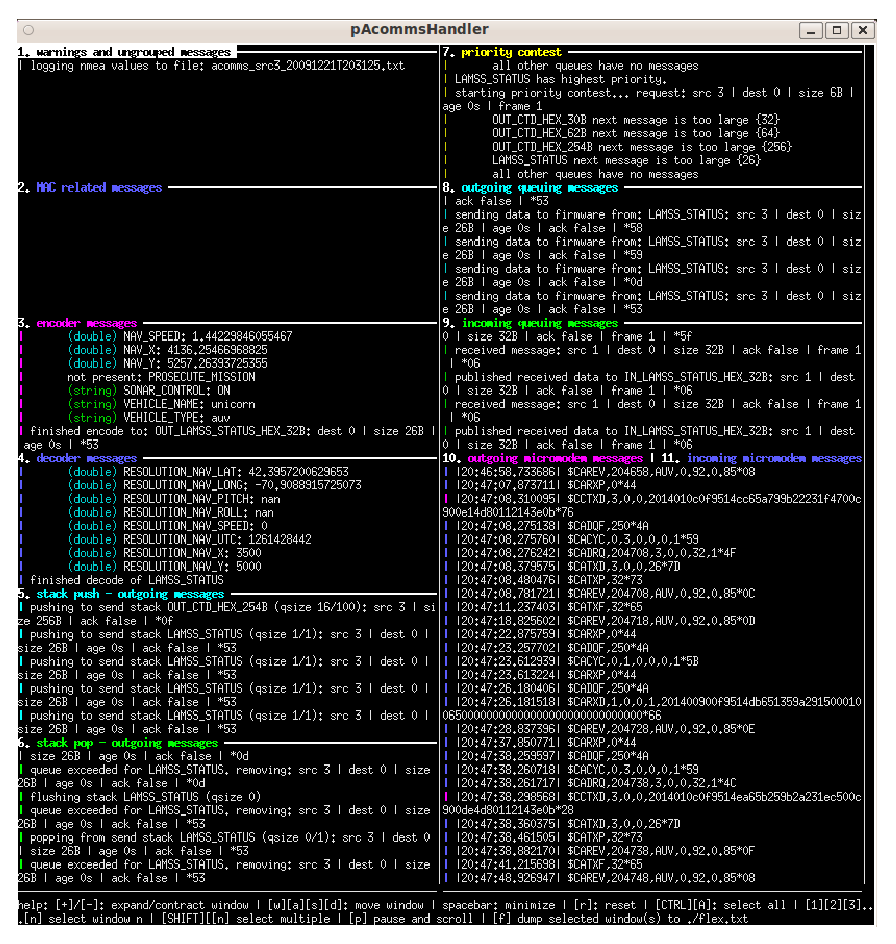
\includegraphics[scale=1]{pAcommsHandler_scope.eps}
\caption{pAcommsHandler running with \texttt{verbosity = scope}. \label{fig:scope}}
\end{figure}

\paragraph{Encoding/Decoding (DCCL) Parameters (\texttt{dccl\_cfg})} \label{dccl_param}
\begin{itemize}
\item \verb|modem_id|: Will be set to the same as \verb|ProcessConfig { modem_id: } |. There is no need to set it again here.
\item \verb|message_file|: \verb|path| to an XML file containing a message set of one or messages. If you want, you can insert one or more manipulators that change the behavior of pAcommsHandler for messages defined in that file. Allowed manipulators:
\begin{itemize}
\item \verb|NO_MANIP|: blank manipulator (behavior is not modified by this manipulator)
\item \verb|NO_ENCODE|: do not encode this message
\item \verb|NO_DECODE|: do not decode this message
\item \verb|NO_QUEUE|: do not queue this message
\item \verb|LOOPBACK|: decode this message internally immediately following encode. Note that messages addressed to the local vehicle are looped back regardless of the value of this manipulator.
\item \verb|ON_DEMAND|: encode immediately preceding  a data request command (use for time sensitive messages like STATUS). This only works if all the message variables are always assumed fresh in the MOOSDB.
\end{itemize}
\item \verb|crypto_password|: optionally provide a password here to encrypt all communications using AES. All receiving nodes must have the same password.
\end{itemize}

\paragraph{Queuing Parameters (\texttt{queue\_cfg})} \label{sec:xmlqueue}
All queue configuration for DCCL messges must be configured within the XML files \verb|<queuing />| tag and included with \verb|message_file: {path: "message.xml"}|. Any \verb|message_file|s specified for \verb|dccl_cfg| are copied to \verb|queue_cfg| and vice-versa, so you don't need to specify them in two places.

CCL messages are configured using the \verb|queue { }| object. The fields for \verb|queue| correspond to the XML \verb|<queuing />| tags:
\begin{itemize}
\item \verb|id|: DCCL: a unique ID for this message (in the range 0-511). CCL: The decimal representation of the first byte of the CCL message to be queued. 
\item \verb|ack|: boolean flag (1=true, 0=false) whether to request an
  acoustic acknowledgment on all sent messages from this field. If
  omitted, default of 0 (false, no ack) is used.
\item \verb|blackout_time|: time in seconds after sending a message
  from this queue for which no more messages will be sent. Use this
  field to stop an always full queue from hogging the channel. If
  omitted, default of 0 (no blackout) is used.
\item \verb|max_queue|: number of messages allowed in the queue before
  discarding messages. If \verb|newest_first| is set to true, the
  oldest message in the queue is discarded to make room for the new
  message. Otherwise, any new messages are disregarded until the space
  in the queue opens up.
\item \verb|newest_first|: boolean flag (1=true=FILO, 0=false=FIFO)
  whether to send newest messages in the queue first (FILO) or not
  (FIFO).
\item \verb|ttl|: the time (in seconds) the message is allowed to live before being discarded. This also factors into the priority calculation as messages with a lower time-to-live (ttl) grow in priority faster. 
\item \verb|value_base|: 
Each queue has a base value ($V_{base}$) and a time-to-live ($ttl$) that create the priority ($P(t)$) at any given time ($t$):
 \[
P(t) = V_{base} \frac{(t-t_{last})}{ttl}
 \]
 where $t_{last}$ is the time of the last send from this queue.

This means for every queue, the user has control over two variables ($V_{base}$ and $ttl$). $V_{base}$ is intended to capture how important the message type is in general. Higher base values mean the message is of higher importance. The $ttl$ governs the number of seconds the message lives from creation until it is destroyed by libqueue. The $ttl$ also factors into the priority calculation since all things being equal (same $V_{base}$), it is preferable to send more time sensitive messages first. So in these two parameters, the user can capture both overall value (i.e. $V_{base}$) and latency tolerance ($ttl$) of the message queue.

\item \verb|in_pubsub_var|: name of the moos variable that is published for received messages to this queue. Not used for DCCL queuing.
\item \verb|out_pubsub_var|: name of the moos variable to subscribe to for
  messages to add to this queue. Not used for DCCL queuing.
\end{itemize}

An example queuing block (for DCCL messages):
\begin{small}
\begin{boxedverbatim}
<message_set>
  <message>
    <id>23</id>
    ...
    <queuing>
      <ack>false</ack>
      <blackout_time>0</blackout_time>
      <max_queue>1</max_queue>
      <newest_first>true</newest_first>
      <value_base>4</value_base>
      <ttl>1000</ttl>
    </queuing>
  </message>
  ...
</message_set>
\end{boxedverbatim}
\resetbvlinenumber
\end{small}

\paragraph{Modem Driver Parameters \texttt{driver\_cfg}}
\begin{itemize}
\item \verb|driver_type|: The only real driver implemented is the \verb|DRIVER_WHOI_MICROMODEM|. \verb|DRIVER_ABC_EXAMPLE_MODEM| is a simple test ``modem''. \verb|DRIVER_NONE| disables the modem driver.
\item \verb|connection_type|: type of connection to make to the modem (\verb|CONNECTION_SERIAL|, \verb|CONNECTION_TCP_AS_CLIENT|, \verb|CONNECTION_TCP_AS_SERVER|).
\item \verb|serial_port|: serial port to which the modem is connected.
\item \verb|serial_baud|: baud rate to use. Should be set to 19200 for the WHOI Micro-Modem.
\item \verb|tcp_port|: networking port to use. 
\item \verb|tcp_server|: IPv4 networking address of the server to connect to. 
\end{itemize}

Extensions for the WHOI Micro-Modem
\begin{itemize}
\item \verb|[MicroModemConfig.nvram_cfg]|: set some modem NVRAM setting to a value. Set \verb|[MicroModemConfig.reset_nvram]: true| to reset all NVRAM (CFG) parameters on startup (\verb|\$CCCFG,ALL,0|). All the \verb|[MicroModemConfig.nvram_cfg]| values are sent after this reset. You do not need to send SRC as this is set to the \verb|modem_id|.
\item  \verb|[MicroModemConfig.hydroid_gateway_id]|: Set to the HYDROID gateway id (1 or 2) \textit{only if using a HYDROID gateway buoy}. Omit for a normal WHOI Micro-Modem.
\end{itemize} 

\paragraph{Medium Access Control (MAC) Parameters \texttt{mac\_cfg}}
\begin{itemize}
\item \verb|mac|: type of Medium Access Control. Values can be \verb|slotted|, \verb|polled|, \verb|fixed_slotted| or \verb|none|.
\item \verb|slot_time|: length, in seconds, of each communication slot for the \verb|mac=slotted| MAC option.
\item \verb|rate|: rate for the \verb|mac=slotted| MAC option. 0 is a single 32 byte packet (FSK), 2 is three frames of 64 bytes (PSK), 3 is two frames of 256 bytes (PSK), and 5 is eight frames of 256 bytes (PSK)
\item \verb|initializer.string|: use the MOOS variable \verb|ACOMMS_MAC_CYCLE_UPDATE| to adjust the TDMA schedule for the  \verb|mac=polled| or \verb|mac=fixed_slotted| MAC option. To set a few initial values, you can use the \verb|initializer| key to ``poke'' this MOOS variable on startup. The format of \verb|ACOMMS_MAC_CYCLE_UPDATE| is a string of comma delimited \verb|key=value| pairs, where \# is an incrementing number for each slot specified in the message. See table \ref{tab:pAcommsHandler:poll} for all the keys and values.

\begin{table}
\centering
\footnotesize
\begin{tabular}{|c|c|c|}
\hline key & value \\ \hline
\hline destination & modem\_id of poller to update  \\ 
\hline update\_type & enum\{add,replace,remove\}  \\ 
\hline slot\_\#\_type & enum\{data,ping\} \\ 
\hline slot\_\#\_from & modem\_id of the sender  \\ 
\hline slot\_\#\_to & modem\_id of the receiver  \\ 
\hline slot\_\#\_rate & rate to poll at  \\ 
\hline slot\_\#\_wait & seconds for the slot to last before next poll \\ 
\hline 
\end{tabular} 
\caption{Parameters of \texttt{mac=polled} and \texttt{mac=fixed\_slotted} reconfiguration message (to \texttt{ACOMMS\_MAC\_CYCLE\_UPDATE})} \label{tab:pAcommsHandler:poll}
\end{table}

for example:
\begin{small}
\begin{boxedverbatim}
destination=1,update_type=add,slot_1_type=data,slot_1_from=1,slot_1_to=0,
slot_1_rate=0,slot_1_wait=15
\end{boxedverbatim}
\resetbvlinenumber
\end{small}

\end{itemize} 

\subsubsection{MOOS variables subscribed to by pAcommsHandler}
\begin{table}
\centering
\footnotesize
\begin{tabular}{|p{0.3\textwidth}|c|p{0.4\textwidth}|p{0.15\textwidth}|}
\hline MOOS variable or .moos file key or XML tag specifying a MOOS variable & Type & Description
& Published by \\  \hline\hline
\textbf{DCCL} &&& \\ \hline\hline
$<$destination\_moos\_var key="destkey"/$>$ & \$ or D & Contains the modem\_id to send this message from. Can either be double (ex: 3) or string (ex: ...,destkey=3,...) & many \\ \hline
$<$trigger\_moos\_var/$>$ & \$ or D & A publish here triggers the creation of this message. The contents may contain message parts or not. & many \\ \hline
$<$moos\_var key="somekey"/$>$ & \$ or D & Data for a given \textit{message\_var}. Can either be double (ex: 3.234) or string (ex: ``bob'' or ``3.234'') or keyed string (ex: ...,somekey=3.234,...). & many \\ \hline
\hline \textbf{Queue} &&& \\ \hline\hline
send= &&&\\  outgoing\_hex\_moos\_var,... & \$ & outgoing\_hex\_moos\_var contains
hexadecimal string to queue (and eventually send). & Various Codecs
(pCTDCodec, pBTRCodec, etc.)\\ \hline
$<$outgoing\_hex\_moos\_var/$>$ & \$ & outgoing\_hex\_moos\_var contains
hexadecimal string to queue (and eventually send). \textbf{Only subscribed for when DCCL encoding is disabled in pAcommsHandler.} & pGeneralCodec \\ \hline
\hline \textbf{Driver} &&& \\ \hline\hline
ACOMMS\_NMEA\_OUT & \$ & Raw messages to send to the modem & \\ \hline
\hline \textbf{MAC} &&& \\ \hline\hline
ACOMMS\_MAC\_CYCLE\_UPDATE & \$ & Updates to the mac=polled or mac=fixed\_slotted TDMA cycle &  \\ \hline
 \end{tabular}
 \caption{MOOS Variables Subscribed to by pAcommsHandler} \label{tab:pAcommsHandler:subscribe}
\end{table}

Some variables are configurable in the .moos file and/or message XML files as described in
section \ref{sec:pAcommsHandler:config}. For example, if
\verb| send = OUT_CTD_HEX_30B, ...| is set in the .moos file (or \\ \verb|<outgoing_hex_moos_var>OUT_CTD_HEX_30B</outgoing_hex_moos_var>| in a message XML file), then
\verb|OUT_CTD_HEX_30B| is the variable actually subscribed. See section \ref{sec:ex_xml} and beyond for details on filling out and interpreting these XML files. See table \ref{tab:pAcommsHandler:subscribe} for a full list of the subscribed variables.

\subsubsection{MOOS variables published by pAcommsHandler}

\begin{table}
\centering
\footnotesize
\begin{tabular}{|p{0.25\textwidth}|c|p{0.4\textwidth}|p{0.2\textwidth}|}
\hline MOOS variable or .moos file key or XML tag specifying a MOOS variable & Type & Description & Format \\ \hline 
\hline \textbf{DCCL} &&& \\ \hline\hline
$<$publish$>$ $<$moos\_var type="string"/$>$ $<$/publish$>$& \$ & (string) Message created from decoded hexadecimal string. & Defined by \xmltag{format} \\ \hline
$<$publish$>$ $<$moos\_var type="double"/$>$ $<$/publish$>$& D & (double) Message created from decoded hexadecimal string. & Defined by \xmltag{format} \\ \hline
$<$outgoing\_hex\_moos\_var/$>$ & \$ & Encoded hexadecimal string. &  \\ \hline
\hline \textbf{Queue} &&& \\ \hline\hline
receive= &&&\\incoming\_hex\_moos\_var,... & \$ & incoming\_hex\_moos\_var contains a hexadecimal string from the micromodem to route to this queue. & see below \\ 
\hline $<$incoming\_hex\_moos\_var/$>$ & \$ & incoming\_hex\_moos\_var contains a hexadecimal string from the micromodem to route to this queue. & see below \\  \hline
ACOMMS\_ACK& \$ & Notification of acknowledged messages &  \\ \hline
ACOMMS\_EXPIRE& \$ & Notification of expired messages (ttl exceeded) &  \\ \hline
ACOMMS\_SQSIZE\_name & \$ & Notification of change in queue size (push or pop) & New size of queue (number of messages) \\ \hline
\hline \textbf{Driver} &&& \\ \hline\hline
ACOMMS\_NMEA\_IN & \$ & Incoming NMEA messages from the modem & See WHOI Micro-Modem Software Interface Guide \\ \hline
ACOMMS\_NMEA\_OUT & \$ & Outgoing NMEA messages to the modem & See WHOI Micro-Modem Software Interface Guide \\ \hline
\hline \textbf{MAC} &&& \\ \hline\hline
 \end{tabular}
 \caption{MOOS Variables Published by pAcommsHandler} \label{tab:pAcommsHandler:publish}
\end{table}

Similarly to the subscriptions, the some publishes done by pAcommsHandler
are defined in the .moos file or in message XML files. Again, instead of MOOS variables,
the table below sometimes indicates the .moos file keys or XML tags for which one can define
the publishes. See table \ref{tab:pAcommsHandler:publish} for a full list of the published variables.

\subsubsection{DCCL Encoding/Decoding Unit: Overview} \label{sec:dccl_overview}

\paragraph{Example message XML file} \label{sec:ex_xml}

 First, let us give a brief background on XML (e\textbf{X}tensible \textbf{M}arkup
 \textbf{L}anguage). XML files contain tags (like
 \xmltag{name}) that are considered ``metadata'' and define both
 the structure of the following data and the contents. Order of the
 tags does not matter for a given level unless explicitly
 specified. Text data resides both in the tags (like
 \xmltag{name$>$bob$<$/name} or as attributes of the tag (such as
 \xmltag{name id="1245"$><$/name}). XML files can be edited with any
 text editor. For more information on XML consult any number of books
 on the subject or browse the internet. XML is a very widely used
 format for storing data that can be both read by both people and
 computers. Also see section \ref{sec:ex} for further examples. Let's call this file example1.xml, which we will use in two following examples:

\begin{small}
\input{includes/example1.xml}
\end{small}

\subsubsection{DCCL Encoding/Decoding Unit: Designing Messages}

\paragraph{Designing a publish triggered message}  \label{sec:design}
We will look at two scenarios and detail how to design a proper message file for each scenario. We will reference the example file given in section \ref{sec:ex_xml} for both scenarios.

Scenario: you want to command an surface craft to move to a new location:
\begin{enumerate}
\item Identify the data: location (x (\verb|goto_x|) and y (\verb|goto_y|) on a local grid). you also want to specify a speed (\verb|goto_speed|) at which it should transit, whether it should have lights (\verb|lights_on|) on or not, and finally a string (\verb|special_instructions|) with possible special instructions. All these data will come in to a moos variable \verb|OUTGOING_COMMAND| on a string like: 
\begin{small}
\begin{boxedverbatim}
OUTGOING_COMMAND: Destination=3,CommandType=GoTo,goto_x=351,goto_y=294,
                  lights_on=true,special_instructions=make_toast,goto_speed=2.3
\end{boxedverbatim}
\resetbvlinenumber
\end{small}
\item Type the data (i.e. is it an int, a float, a string?) and give the ranges and precisions needed: 
\begin{itemize}
\item \verb|goto_x|: integer (in meters) (\verb|int|) that will operate on a (positive valued) local grid not to exceed 10 km in either dimension. 
\item \verb|goto_y|: same as \verb|goto_x|.
\item \verb|goto_speed|: speed in m/s. the vehicle cannot exceed 3 m/s and does not go backwards. we would like to give precise speeds to the hundredths place. thus, we need a \verb|float| ranging from 0 to 3 with precision 2.
\item \verb|lights_on|: simply a flag (boolean value) whether to have our lights on or off. thus, we need a \verb|bool| \textit{message\_var}.
\item \verb|special_instructions|: We want a field that can hold any string of characters, but we know it will not exceed ten characters. thus, we need a \verb|string| \textit{message\_var}.
\end{itemize}
\item Putting all this together, we can define the \xmltag{layout} portion of the first message defined in section \ref{sec:ex_xml}. We do not need any \xmltag{moos\_var} tags within the \textit{message\_var}s since all the data are contained in the contents of the trigger variable message (\verb|OUTGOING_COMMAND|). That is, when we leave out the \xmltag{moos\_var}, pGeneralCodec will insert \xmltag{moos\_var$>$OUTGOING\_COMMAND$<$/moos\_var}, which is exactly what we want. For example, taking one of the \textit{message\_var}s:
\begin{small}
\begin{boxedverbatim}
      <int>
        <name>goto_x</name>
        <max>10000</max>
        <min>0</min>
      </int>
\end{boxedverbatim}
\resetbvlinenumber
\end{small}
is exactly the same as saying 
\begin{small}
\begin{boxedverbatim}
      <int>
        <name>goto_x</name>
        <moos_var>OUTGOING_COMMAND</moos_var>
        <max>10000</max>
        <min>0</min>
      </int>
\end{boxedverbatim}
\resetbvlinenumber
\end{small}

\item Now we can fill out the rest of the tags on the \xmltag{message} level:
\begin{itemize}
\item \xmltag{name$>$GoToCommand$<$/name}: just a name so we can identify this message quickly when reading through the XML.
\item \xmltag{outgoing\_hex\_moos\_var$>$OUT\_GOTO\_HEX$<$/outgoing\_hex\_moos\_var}: we will publish our hex strings here for consumption by the low level modem stack processes (probably pAcommsHandler \verb|send=OUT_GOTO_HEX...|). the publishes will look a bit like:
\begin{small}
\begin{boxedverbatim}
OUT_GOTO_HEX: Dest=3,HexData=a9385bc098109830a9385bc0981098a9385bc098109830a9385bc0981098
\end{boxedverbatim}
\resetbvlinenumber
\end{small}

\item \xmltag{incoming\_hex\_moos\_var$>$IN\_GOTO\_HEX$<$/incoming\_hex\_moos\_var}: where we expect to receive incoming messages to decode (probably from pAcommsHandler \verb|receive=IN_GOTO_HEX...|). messages should be pure hex with the community set to the sending \textit{modem\_id}. An example for the received message on \textit{modem\_id}=3 if the sending node (say a topside command computer) is \textit{modem\_id}=1:
\begin{small}
\begin{boxedverbatim}
IN_GOTO_HEX: a9385bc098109830a9385bc0981098a9385bc098109830a9385bc0981098 
{Community=1}
\end{boxedverbatim}
\resetbvlinenumber
\end{small}
\item \xmltag{trigger$>$publish$<$/trigger}: we are creating this message on a \textbf{publish} (to \verb|OUTGOING_COMMAND|).
\item \xmltag{trigger\_moos\_var mandatory\_content="CommandType=GoTo"$>$OUTGOING\_COMMAND$<$/trigger\_moos\_var}: \verb|OUTGOING_COMMAND| is the trigger variable and it must contain the substring \verb|CommandType=GoTo|. That is, other commands might be published here (e.g. \verb|CommandType=Loiter|, \verb|CommandType=Track|) and we do not define the message structure of those here (this particular \xmltag{message$><$/message} is only for a GoTo message). Other messages can be created to encode/decode these other command types.
\item \xmltag{size$>$30$<$/size}: we want this message to fit in a WHOI micromodem FSK frame (32 bytes) and thus we have 30 bytes to work with (pAcommsHandler needs 2 bytes of header).
\end{itemize}
\item Finally, we fill out the \xmltag{publish} section which indicates where (i.e. what moos variables) and how (what format and which part(s) of the message) pGeneralCodec should publish decoded messages upon receipt of hex from other vehicles. Each \xmltag{publish} indicates a separate action that is taken upon receipt of a message. As many \xmltag{publish} sections as desired may be included for a given message. So, for our example message, we want to replicate the original string (a common practice):
\begin{small}
\begin{boxedverbatim}
INCOMING_COMMAND: CommandType=GoTo,goto_x=351,goto_y=294,
                  lights_on=true,special_instructions=make_toast,goto_speed=2.3
\end{boxedverbatim}
\resetbvlinenumber
\end{small}
to do this we fill out a publish \xmltag{all}. This is the simplest form of the \xmltag{publish} section:
\begin{small}
\begin{boxedverbatim}
    <on_receipt>
      <publish>
        <moos_var>INCOMING_COMMAND</moos_var>
        <all />
      </publish>
    </on_receipt>
\end{boxedverbatim}
\resetbvlinenumber
\end{small}
this says to take every \textit{message\_var} and make a ``key=value'' comma-delimited string from it. the above \xmltag{publish} block is a shortcut for a much longer form:
\begin{small}
\begin{boxedverbatim}
    <on_receipt>
      <publish>
        <moos_var>INCOMING_COMMAND</moos_var>
        <format>type=goto,goto_x=%1%,goto_y=%2%,lights_on=%3%,
        special_instructions=%4%,goto_speed=%5%</format>
        <message_var>goto_x</message_var>
        <message_var>goto_y</message_var>
        <message_var>lights_on</message_var>
        <message_var>special_instructions</message_var>
        <message_var>goto_speed</message_var>
      </publish>
    </on_receipt>
\end{boxedverbatim}
\resetbvlinenumber
\end{small}
These two blocks are functionally identical.

We may want to also publish the \verb|special_instructions| to another moos variable, so that:
\begin{small}
\begin{boxedverbatim}
SPECIAL_INSTRUCTIONS: special_instructions=make_toast,lights_on=true
\end{boxedverbatim}
\resetbvlinenumber
\end{small}
we can do this with another publish block:
\begin{small}
\begin{boxedverbatim}
    <publish>
      <moos_var>SPECIAL_INSTRUCTIONS</moos_var>
      <format>special_instructions=%1%,lights_on=%2%</format>
      <message_var>new_instructions</message_var>
      <message_var>lights_on</message_var>
    </publish>
\end{boxedverbatim}
\resetbvlinenumber
\end{small}
in this case the \xmltag{format} block is necessary because the default would be \\ 
\xmltag{format$>$new\_instructions=\%1\%,lights\_on=\%2\%$<$/format} not \\
\xmltag{format$>$special\_instructions=\%1\%,lights\_on=\%2\%$<$/format}.
\end{enumerate}

Those are the basics to designing a \textbf{publish} triggering message.

\paragraph{Designing a time triggered message}
Scenario: we need a status message that grabs data from various moos variables and publishes them (encoded) on a time interval. We will not go into as much detail here, but rather highlight the changes from the previous scenario.
\begin{itemize}
\item you will notice
\begin{small}
\begin{boxedverbatim}
    <trigger>time</trigger>
    <trigger_time>30</trigger_time>
\end{boxedverbatim}
\resetbvlinenumber
\end{small}
instead of 
\begin{small}
\begin{boxedverbatim}
    <trigger>publish</trigger>
    <trigger_moos_var mandatory_content="CommandType=GoTo">OUTGOING_COMMAND</trigger_moos_var>
\end{boxedverbatim}
\resetbvlinenumber
\end{small}
this indicates that a message should be made on a time interval (given by \xmltag{trigger\_time}, which is every 30 seconds here), rather than on a publish to some moos variable.
\item you will notice that all the \textit{message\_var}s have a \xmltag{moos\_var} tag, which was omitted in the previous example since we were taking data from the trigger variable. Obviously, there is no trigger variable now so we must specify a location for the data to come from (in the moos db). The newest available value will be used when the message needs to be made. This means there is no guarantee that the data is fresh. Thus, you should use moos variables that are often updated for a \xmltag{trigger$>$time$<$/trigger} message. If this is not the case, a \xmltag{trigger$>$publish$<$/trigger} message (see previous scenario) may be a better choice.
\item the format of the value read from the \xmltag{moos\_var} can have several options. First, if the \textit{message\_var} is of a numeric type (\xmltag{int}, \xmltag{float}, \xmltag{bool}) and the \xmltag{moos\_var} is a double, the value of the double is used as is (with appropriate rounding and type casting). If the \textit{message\_var} is a string, two options are available. First, the pGeneralCodec looks for a substring of the form:
\begin{small}
\begin{boxedverbatim}
name=value
\end{boxedverbatim}
\resetbvlinenumber
\end{small}
within the string and picks out the value to send for the message. If there is no such \verb|name=| substring, the entire string is converted to the appropriate form. An example: we have a \xmltag{float} called \xmltag{name$>$my\_float$<$/name} that has a tag \xmltag{moos\_var$>$SOME\_FLOAT\_VARIABLE$<$/moos\_var}: 
\begin{itemize}
\item if
\begin{small}
\begin{boxedverbatim}
(double)SOME_FLOAT_VARIABLE: 3.56
\end{boxedverbatim}
\resetbvlinenumber
\end{small}
then 3.56 is sent.
\item if instead 
\begin{small}
\begin{boxedverbatim}
(string)SOME_FLOAT_VARIABLE: "my_float=3.56"
\end{boxedverbatim}
\resetbvlinenumber
\end{small}
then 3.56 is still sent.
\item if instead
\begin{small}
\begin{boxedverbatim}
(string)SOME_FLOAT_VARIABLE: "3.56"
\end{boxedverbatim}
\resetbvlinenumber
\end{small}
again, 3.56 is sent.
\item Finally, if some other string like
\begin{small}
\begin{boxedverbatim}
(string)SOME_FLOAT_VARIABLE: "blah=3.56"
\end{boxedverbatim}
\resetbvlinenumber
\end{small}
then \verb|blah=3.56| is converted (using streams) to a float, which will probably be zero or something else undesired. In other words, this case is not what you want, whereas the above three are fine.
\end{itemize}
\end{itemize}
\paragraph{Further examples} \label{sec:ex}
\begin{itemize}
\item I currently store our working message files in \verb|moos-ivp-local/data/acomms|. look for .xml files in this directory for further examples.
\item Probably the simplest message you can make (for a single string MOOS variable published to \verb|MY_STRING| that gets truncated at 30 chars (need two bytes for CCL and DCCL ids) and sent to broadcast):
\begin{small}
\begin{boxedverbatim}
<?XML version="1.0" encoding="UTF-8"?>
<message_set>
  <message>
    <name>SimpleStringSender</name>
    <id>1</id>    
    <trigger>publish</trigger>
    <trigger_moos_var>MY_STRING</trigger_moos_var>
    <size>32</size>
    <layout>
      <string>
        <name>my_string</name>
        <max_length>30</max_length>
      </string>
    <on_receipt>
      <publish>
        <moos_var>INCOMING_COMMAND</moos_var>
        <all />
      </publish>
    <on_receipt>
  </message>
</message_set>
\end{boxedverbatim}
\resetbvlinenumber
\end{small}
\end{itemize}


\subsubsection{DCCL Encoding/Decoding Unit: XML Tag Reference}

\begin{figure}
\centering
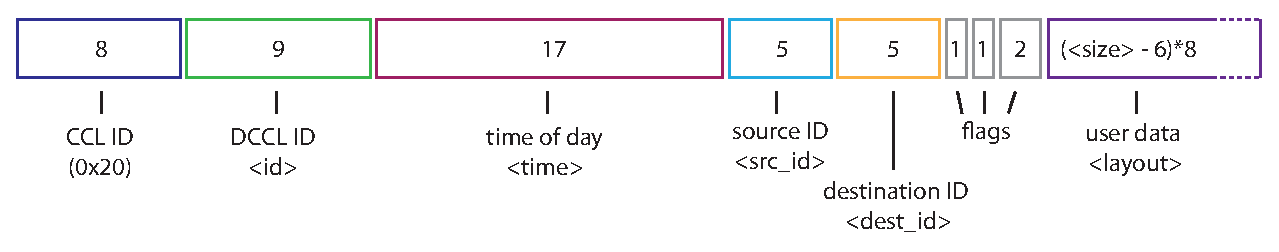
\includegraphics[width=0.8\textwidth]{dccl-header.eps}
\caption{Layout of the DCCL header, showing the fixed size (in bits) of each header field. The user cannot modify the size of these header fields, but can access and set the data inside through the same methods used for the customizable data fields specified in \xmltag{layout}. The flags are not used by DCCL, but are included for use by the lower level networking.}
\label{fig:header}
\end{figure}

\paragraph{Message XML file reference: allowed tags} Let us now give a description of all the allowed tags:

\begin{itemize}
\item \xmltag{?xml version="1.0" encoding="UTF-8"?}: specifies the file is XML. All you need to know is that this must be the first line of every message XML file.
\item \xmltag{message\_set}: the root element. All XML files must have a single root element. Since we are define a set of messages (one or more per file), this is a logical choice of name for the root element. [mandatory, one allowed].
\item \xmltag{message}: defines the start of a message. [mandatory, one or more allowed].
\begin{itemize}
\item \xmltag{name}: a human readable name for the message. This is not used internally at this point in time. [mandatory, one allowed]
\item \xmltag{size}: the maximum allowed size of the message in bytes. There are eight bits (binary digits) to a byte. Use $N$ here for messages passed to the micromodem where $N$ is the desired micromodem frame size ($N=$32, 64, or 256 depending on the rate). If the \xmltag{layout} of the message exceeds this size, pAcommsHandler will exit on startup with information about sizes, from which you can remove or reduce the size of certain \textit{message\_var}s.
\item \xmltag{repeat}: make as many copies of the message structure defined in \xmltag{layout} as will fit in the message \xmltag{size}. No message will be sent until the message is full. For example, if the message is 32 bytes and the layout is 8 bytes, three copies of the message will be stored before sending ($32-6-3*8 = 0$). That is, three messages will be triggered, packed and sent as a single DCCL message. [optional, if omitted only a single copy is made]. \textit{If \xmltag{repeat} is specified, \textit{array\_length} must omitted for all \textit{message\_vars}}. That is, you cannot have repeated messages that contain arrays.
\item \xmltag{header}: the children of this tag allow the user to rename the header parts of the DCCL message. See Fig.~\ref{fig:header} for a sketch of the DCCL header format. These names are used when passing values at encode time for the various header fields.
\begin{itemize}
\item \xmltag{id}: an unsigned nine bit integer (1-511) that identifies this message within a network. very similar to the CCL identifier, but for DCCL messages. The CCL identifier occupies the most significant byte (MSB) of the message followed by this id which takes the second MSB. \textit{This must be unique within a network as this id determines the message decoding} [mandatory, one allowed]
\item \xmltag{time}: seconds elapsed since 1/1/1970 (``UNIX time''). In the DCCL encoding, this reduced to seconds since the start of the day, with precision of one second. Upon decoding, assuming the message arrives within twelve hours of its creation, it is properly restored to a full UNIX time.
\begin{itemize}
\item \xmltag{name}: the name of this field; optional, the default is ``\_time''. [\verb|string|]
\end{itemize}
\item \xmltag{src\_id}: a unique address (\xmltag{src\_id} $\in [0,31]$) of the sender of this message. For a given experiment these short unique identifiers can be mapped on to more global keys (such as vehicle name, type, ethernet MAC address, etc.).
\begin{itemize}
\item \xmltag{name}: default is ``\_src\_id''. [\verb|string|]
\end{itemize}
\item \xmltag{dest\_id}: the eventual destination of this message (also an \verb|unsigned integer| in the range [0,31]). If this destination exists on the same subnet as the sender, this will also be the hardware layer destination id number.
\begin{itemize}
\item \xmltag{name}: default is ``\_dest\_id''. [\verb|string|]
\end{itemize}
\end{itemize}
\item \xmltag{layout}: defines the message structure itself (what fields [the message variables or \textit{message\_var}s] the message contains and how they are to be encoded). [mandatory, one allowed].
\begin{itemize}
\item \xmltag{static}: a \textit{message\_var} that is not actually sent with the message but can be used to include in received messages (\textit{publishes}). [optional, one or more allowed]. 
\begin{itemize}
\item \xmltag{name}: the name of this \textit{message\_var}. [mandatory, one allowed].
\item \xmltag{value}: the value of this static variable. [mandatory, one allowed].
\end{itemize}
\item \xmltag{bool algorithm=""}: a boolean (true or false) \textit{message\_var}  The optional parameter \verb|algorithm| allows you to perform certain algorithms on the data before encoding. See below. [optional, one or more allowed]. 
\begin{itemize}
\item \xmltag{name}
\item \xmltag{moos\_var}: the moos variable from which to pull the value of this field. [optional if \xmltag{trigger$>$publish$<$/trigger}: default is trigger\_moos\_var; mandatory if \xmltag{trigger$>$time$<$/trigger}, one allowed]. 
\item \xmltag{array\_length}: if larger than 1, this makes a bool array instead of a single bool. [optional, default is  1].
\end{itemize}
\item \xmltag{int algorithm=""}: an integer \textit{message\_var} [optional, one or more allowed]. 
\begin{itemize}
\item \xmltag{name}
\item \xmltag{moos\_var}
\item \xmltag{max}: the maximum value this field can take. [mandatory, one allowed].
\item \xmltag{min}: the minimum value this field can take. [mandatory, one allowed].
\item \xmltag{array\_length}
\item \xmltag{max\_delta}: if specified, delta-difference encoding is done of the \xmltag{repeat}ed message or the values in the array (for \xmltag{array\_length} $>$ 1). The first value is used as a key for the remaining values which are sent as a difference to this key. The number specified here is the maximum expected difference between the first value (key) and any of the remaining values in the message. [optional, if omitted, delta-difference encoding is not performed].
\end{itemize}
\item \xmltag{float algorithm=""}: a floating point \textit{message\_var} [optional, one or more allowed].
\begin{itemize}
\item \xmltag{name}
\item \xmltag{moos\_var}
\item \xmltag{max}
\item \xmltag{min}
\item \xmltag{precision}: an integer that specifies the number of decimal digits to preserve. Negatives are allowed. For example, \xmltag{precision$>$2$<$/precision} rounds 1042.1234 to 1042.12; \xmltag{precision$>$-1$<$/precision} rounds 1042.1234 to 1.04e3. [mandatory, one allowed].
\item \xmltag{array\_length}
\item \xmltag{max\_delta}
\end{itemize}
\item \xmltag{string algorithm=""}: an ASCII string \textit{message\_var} [optional, one or more allowed].
\begin{itemize}
\item \xmltag{name}
\item \xmltag{moos\_var}
\item \xmltag{max\_length}: the length of the string value in this field. Longer strings are truncated. \xmltag{max\_length$>$4$<$/max\_length} means ``ABCDEFG'' is sent as ``ABCD''. [mandatory, one allowed].
\item \xmltag{array\_length}
\end{itemize}
\item \xmltag{enum algorithm=""}: an enumeration \textit{message\_var} [optional, one or more allowed].
\begin{itemize}
\item \xmltag{name}
\item \xmltag{moos\_var}
\item \xmltag{value}: a possible value (string) the enum can take. Any number of values can be specified. [mandatory, one or more allowed].
\item \xmltag{array\_length}
\end{itemize}
\item \xmltag{hex}: a message variable represented pre-encoded hexadecimal to add to the message. This field is useful if another source is encoding part or all of a DCCL message. [optional, one or more allowed]. 
\begin{itemize}
\item \xmltag{name}: the name of this \textit{message\_var}. [mandatory, one allowed].
\item \xmltag{moos\_var}
\item \xmltag{num\_bytes}: the number of bytes for this field. The string provided should be twice as many characters as \xmltag{num\_bytes} since each character of a hexadecimal string is one nibble (4 bits or 1/2 byte). [mandatory, one allowed].
\item \xmltag{array\_length}
\end{itemize}
\end{itemize}
\item \xmltag{on\_receipt}: begins a set of actions to be performed when a message of this type is received from another vehicle. [mandatory, one allowed].
\begin{itemize}
\item \xmltag{publish}: defines a single output value upon receipt of a message. Any number of publishes containing any subset of the \textit{message\_var}s can be specified. [mandatory, one or more allowed].
\begin{itemize}
\item \xmltag{moos\_var}: the name of the moos variable to publish to. If desired, a format string is allowed here as well (e.g. \verb|\%1\%_NAV_X| will fill \verb|\%1\%| with the first \textit{message\_var}). See the \xmltag{format} tag description for more info. [mandatory, one allowed].
\item \xmltag{format}: a string conforming to the format string syntax of the boost::format \footnote{see the syntax of the \textbf{format-string} at \textit{http://www.boost.org/doc/libs/1\_37\_0/libs/format/doc/format.html\#syntax}} library. This field will specify the format of the string published to the moos variable defined in \xmltag{moos\_var}. At its simplest it is a string of incrementing numbers surrounded by \%\%. Or, instead, you may also use a printf style string, using \%d for int  \textit{message\_var}, \%lf for floats, and \%s for strings, bools and enums. [optional: default is \verb|name1=\%1\%,name2=\%2\%,name3=\%3\%|, where \verb|name1| is the name of the first \xmltag{message\_var} field to follow, \verb|name2| is the second, etc. exception: default is \verb|\%1\%| if only a single \xmltag{message\_var} defined. one allowed].
\item \xmltag{message\_var algorithm=""}: the name (\xmltag{name} above) of a \textit{message\_var} contained in this message (i.e. an \xmltag{int}, \xmltag{bool}, etc.) the values of these fields upon receipt of a message will be used to populate the format string and the result will be published to \xmltag{moos\_var}. The optional parameter \verb|algorithm| allows you to perform certain algorithms on the data after receipt before publishing. See below. [mandatory unless \xmltag{all} used, one or more allowed].
\item \xmltag{all}: equivalent to \xmltag{message\_var} for all the \textit{message\_var}s in the message. This is a shortcut when you want to publish all the data in a human readable string. [optional, one allowed].
\end{itemize}
\end{itemize}
\item \xmltag{queuing}: optional section used by pAcommsHandler to handle message queuing. See section \ref{sec:xmlqueue} for details.
\item \xmltag{trigger}: how the message is created. Currently this field must take the value ``publish'' (meaning a message is created on a publish event to a certain moos variable) or ``time'' (a message is created on a certain time interval). [mandatory, one allowed]
\item \xmltag{trigger\_var}: used if \xmltag{trigger$>$publish$<$/trigger}, this field gives the MOOS variable that publishes to will trigger the creation of this message [mandatory if and only if \xmltag{trigger$>$publish$<$/trigger}]. optional attribute \verb|mandatory_content| specifies a string that must be a substring of the contents of the trigger variable in order to trigger the creation of a message. For example, if you wanted to create a certain message every time \verb|COMMAND| contained the string \verb|CommandType=GoTo...| but no other time, you would specify \\ \verb|mandatory_content="CommandType=GoTo"| within this tag.
\item \xmltag{trigger\_time}: used if \xmltag{trigger$>$time$<$/trigger}, this field gives the time interval pGeneralCodec should create this message. For example, a value of \\ \xmltag{trigger\_time$>$10$<$/trigger\_time} would mean a message was created every ten seconds. [mandatory if and only if \xmltag{trigger$>$time$<$/trigger}].
\item \xmltag{destination\_var}: moos variable to find where this message should be sent. Specify attribute ``key='' to specify a substring to look for within the value of this moos variable. For example, if \verb|COMMAND| contained the string \verb|Destination=3| and you want this message sent to modem\_id 3, then you should set \verb|key=Destination| to properly parse that string. [optional: default is 0 (broadcast), one allowed].
\item \xmltag{incoming\_hex\_moos\_var}: where to look for messages (hex string) to decode. [optional, one allowed. default is \verb|IN_<name/>_HEX_<size/>B|].
\item \xmltag{outgoing\_hex\_moos\_var}: where to publish the encoded message (as a hexadecimal string). [optional, one allowed. default is \verb|OUT_<name/>_HEX_<size/>B|].
\end{itemize}
\end{itemize}

\paragraph{Algorithms}
You can perform a number of simple algorithms on data either before encoding (specified in the \textbf{message\_var} tag (e.g. \xmltag{string algorithm=""}) or after receipt (specified in the \xmltag{message\_var} tag. You can apply more than one algorithm by separating them with commas and they are processed in the order given. The currently implemented algorithms include:
\begin{itemize}
\item \verb|to_upper|: converts string, enum, or bool to uppercase
\item \verb|to_lower|: converts string, enum, or bool to lowercase
\item \verb|angle_0_360|: wraps float or int angle in degrees into the range of [0, 360)
\item \verb|angle_-180_180|: wraps float or int angle in degrees into the range of [-180, 180)
\item \verb|lon2utm_x|: converts longitude to a local utm coordinate (meters) used by LAMSS\footnote{we define a latitude/longitude origin near our basis of operations. From this datum we calculate the UTM northings (y) and eastings (x). All further UTM calculations are the offset from this datum point. This offset is what is returned by this algorithm. Contact me if you need more information on this.}. Requires \verb|LatOrigin| and \verb|LongOrigin| to be specified at the top of the moos file. Since a UTM conversion requires a lon/lat pair, you must specify the latitude variable here to pair with by adding a colon after this algorithm followed by the name of the latitude variable. e.g. \xmltag{message\_var algorithm="lon2utm\_x:our\_lat"$>$our\_lon$<$/message\_var} converts \verb|our_lon| to a local x (easting) using \verb|our_lat| as the latitude point.
\item \verb|lat2utm_y|: similar to \verb|lon2utm_x| but for latitude. \\ e.g. \xmltag{message\_var algorithm="lat2utm\_y:our\_lon"$>$our\_lat$<$/message\_var} converts \verb|our_lat| to a local y (northing) using \verb|our_lon| as the longitude point.
\item \verb|utm_x2lon|: the reverse conversion from x to longitude. similarly to the latitude, longitude to x,y conversion you must pair x and y. e.g., \\ \xmltag{message\_var algorithm="utm\_x2lon:our\_y"$>$our\_x$<$/message\_var}
\item \verb|utm_y2lat|: example: \xmltag{message\_var algorithm="utm\_y2lat:our\_x"$>$our\_y$<$/message\_var}
\item \verb|modem_id2name|: converts a WHOI modem\_id to a vehicle name. requires a file (path given in the .moos as \verb|modem_id_lookup_path=/path/to/modemidlookup.txt|. an example file:
\begin{boxedverbatim}
// modem_id, vehicle name (should be community name), vehicle type, other aliases
0, broadcast, broadcast
1, endeavor, ship
3, unicorn, auv
4, macrura, auv
\end{boxedverbatim}
\resetbvlinenumber
if no match is found, the modem\_id is returned as a string (e.g. "10").
\item \verb|name2modem_id|: performs the (case insensitive) reverse lookup on the same file. if no match is found, \verb|atoi(name.c_str())| is returned (probably zero unless you passed something like "4" to this function).
\item \verb|modem_id2type|: similar to \verb|modem_id2name| but returns the type of the vehicle (ship, auv, etc.)
\item \verb|power_to_dB|: takes $10\log_{10}$ of the value.
\item \verb|dB_to_power|: takes power antilog of the value.
\item \verb|alg_TSD_to_soundspeed|: applied to temperature, with references to salinity and depth, calculates the speed of sound using the Mackenzie equation. For example: \xmltag{message\_var algorithm="alg\_TSD\_to\_soundspeed:sal:depth"$>$temp$<$/message\_var}
\item \verb|add|: adds the reference \xmltag{message\_var} to the current \xmltag{message\_var}. example: \xmltag{message\_var algorithm="add:b"$>$a$<$/message\_var} adds b to a.
\item \verb|subtract|: subtracts the reference \xmltag{message\_var} from the current \xmltag{message\_var}.
\end{itemize}

\subsubsection{DCCL Encoding/Decoding Unit: Under the Hood}

\paragraph{Bitwise Layout of the Messages}

We may want to know the actual layout of the binary/hex message. Let us explain it with an example; for the first example message in \verb|example1.xml| given in section \ref{sec:ex_xml}, if we run pGeneralCodec we get information about that message:
\begin{small}
\begin{boxedverbatim}
        type (static):
                value: {goto}
                size [bits]: [0]
        goto_x (int):
                source: {OUTGOING_COMMAND}
                [min, max] = [0,10000]
                size [bits]: [14]
        goto_y (int):
                source: {OUTGOING_COMMAND}
                [min, max] = [0,10000]
                size [bits]: [14]
        lights_on (bool):
                source: {OUTGOING_COMMAND}
                size [bits]: [1]
        new_instructions (string):
                source: {SPECIAL_INSTRUCTIONS}
                max_length: {10}
                size [bits]: [80]
        goto_speed (float):
                source: {OUTGOING_COMMAND}
                [min, max] = [0,3]
                precision: {2}
                size [bits]: [9]
\end{boxedverbatim}
\resetbvlinenumber
\end{small}
the calculated sizes are used to pack the message like so (\verb|{\#}| equals size of field in bits), where left to right is the same as reading the hex string from left to right:
\begin{small}
\begin{boxedverbatim}
[[0 {122}][goto_x {14}][goto_y {14}][lights_on {1}][new_instructions {80}][goto_speed {9}]]
\end{boxedverbatim}
\resetbvlinenumber
\end{small}
where \verb|[0 {122}]| means zero fill the front of the message to the full size (30 bytes = 240 bits minus 118 for other fields = 122). Byte boundaries are dissolved and encoded as a string ``ABCDEF...'' where the most significant byte (MSB, or leftmost 8 bits) is 0xAB, second MSB is 0xCD, etc. 


The encoding of each \textit{message\_var} is done as an unsigned integer, with the exception of strings, which are store as ASCII. The value 0 (all bits zero) always indicates "not specified" or "Not a Number" (nan). This means that the user did not specify any value for this field, specified a value causing overflow (\xmltag{int} or \xmltag{float} greater than \xmltag{max} or less than \xmltag{min}), or provided a value for an \xmltag{enum} that did not match any of the enumerate's \xmltag{value} options. Along with this rule, the method for encoding and decoding is given in Table \ref{tab:dccl_enc}. An example is provided in Fig. \ref{fig:dccl_example}. 

\begin{table}[!t]
\centering
\begin{threeparttable}
\setlength{\extrarowheight}{2pt}
\caption{Formulas for encoding the DCCL types.}
\label{tab:dccl_enc}
\begin{tabular}{m{0.1\textwidth}|m{0.3\textwidth}|m{0.5\textwidth}}
\hline DCCL Type & Size (bits) & Encode\tnote{a}  \\ \hline
\hline \xmltag{bool} & 2 & 
$x_{enc} = \left\{ 
\begin{array}{l l}
  2 & \quad \text{if $x$ is true}\\
  1 & \quad \text{if $x$ is false}\\
  0 & \quad \text{if $x$ is undefined}\\
\end{array} \right.$
\\ 
\hline \xmltag{enum} & $\lceil \hbox{log}_2(1+\sum{\epsilon_i}) \rceil$ & $x_{enc} =  \left\{ 
\begin{array}{l l}
  i+1 & \quad \text{if $x \in \{\epsilon_i\}$ }\\
  0 & \quad \text{otherwise}\\
\end{array} \right.$   \\ 
\hline \xmltag{string} & $length \cdot 8$ & ASCII\tnote{b} \\ 
\hline \xmltag{int} & $\lceil \hbox{log}_2(max-min + 2) \rceil$ & $x_{enc} =  \left\{ 
\begin{array}{l l}
  \hbox{nint}(x - min) + 1  & \quad \text{if $x \in [min,max]$ }\\
  0 & \quad \text{otherwise} \\
\end{array} \right.$   \\ 
\hline \xmltag{float} & $\lceil \hbox{log}_2((max-min)\cdot 10^{precision} + 2) \rceil$ &  $x_{enc} =  \left\{ 
\begin{array}{l l}
  \hbox{nint}((x - min)\cdot 10^{precision})+1 & \quad \text{if $x \in [min,max]$ }\\
  0 & \quad \text{otherwise} \\
\end{array} \right.$   \\ 
\hline \xmltag{hex} & $num\_bytes \cdot 8$ & $x_{enc}$ = $x$ \\ 
\hline 
\end{tabular}
\begin{tablenotes}
\item $\cdot$ $x$ is the original (and decoded) value; $x_{enc}$ is the encoded value. 
\item $\cdot$ $min$, $max$, $length$, $precision$, $num\_bytes$ are the contents of the \xmltag{min}, \xmltag{max}, \xmltag{max\_length}, \xmltag{precision}, and \xmltag{num\_bytes} tags, respectively. $\epsilon_i$ is the $i$th \xmltag{value} child of the \xmltag{enum} tag (where $i = 0, 1, 2, \ldots$).
\item $\cdot$ nint($x$) means round $x$ to the nearest integer.
\item[a] for all types except \xmltag{string} and \xmltag{hex}, if data are not provided or they are out of range (e.g. $x > max$), they are encoded as zero ($x_{enc} = 0$) and decoded as not-a-number (NaN).
\item[b] the end of the string is padded with zeros to $length$ before encoding if necessary.
\end{tablenotes}
\end{threeparttable}
\end{table}


\begin{figure}
\centering
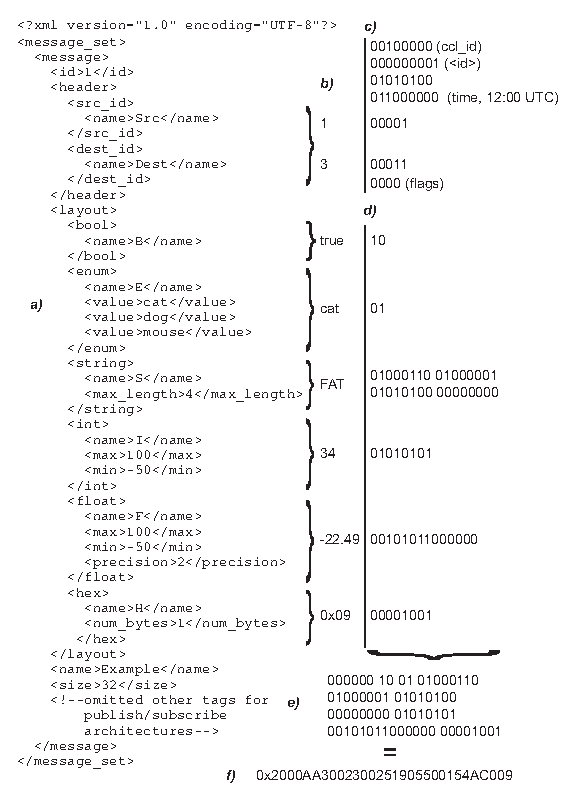
\includegraphics[width=0.8\textwidth]{dccl_example}
\caption{Example of the DCCL encoding process. The process of encoding starts with the DCCL XML file (a). Data are provided by the application (b). \textit{libdccl} encodes these data to binary via the algorithms given in Table~\ref{tab:dccl_enc} to form the header (c) and layout (d), concatenates and zero fills the encoded layout from most significant bit to closest byte (e) to produce the full encoded message (f). Finally, this point the message is encrypted (if desired). }
\label{fig:dccl_example}
\end{figure}




%\paragraph{Message XML reference sheet}
%This is a quick reference of all the allowed tags with some comments about their use:
%
%\begin{small}
%\input{includes/message_xml_cheatsheet.xml}
%\end{small}

\subsubsection{Priority Message Queuing Unit}

pAcommsHandler takes all the configured queues and maintains a stack of messages for each
  queue. when it is prompted by data by iMicroModem, it has a priority
  "contest" between the queues. the queue with the current highest
  priority (as determined by the \verb|priority| and
  \verb|priority_time_const| fields) is selected. The next message in
  that queue is then provided to the MicroModem to send. For modem
  messages with multiple frames per packet, each frame is a separate
  contest. Thus a single packet may contain frames from different
  queues (e.g. a rate 5 PSK packet has eight 256 byte frames. frame 1
  might grab a STATUS message since that has the current highest
  queue. then frame 2 may grab a BTR message and frames 3-8 are filled
  up with CTD messages (e.g. STATUS is in blackout, BTR queue is
  empty)).

For messages with \verb|ack=1| (acknowledge requested), the last
  message continues to be re-sent (that is, it is not popped from the
  message queue) until the ACK is received from the modem (thus
  blocking the sending of other messages). Perhaps i will add max
  retries at some point soon. Messages with \verb|ack=0| are popped
  and discarded when they are sent (no retries).

If you do not wish for dynamic growth of the priorities, simply
  set the \verb|ttl| to the special value 0. Then the priorities grow as $P = V\_{base}$ and messages never expire. Note that this is the same as setting \verb|ttl| = $\infty$.

\paragraph{Messages not to us are ignored} We choose modem id 0 as broadcast. thus messages with the destination
  field = 0 will always be read by all nodes and reported to the
  appropriate moos variable. Otherwise, we ignore messages unless they
  correspond to our modem id. so if you send a message to modem id 10,
  pAcommsHandler for modem ids $1 \rightarrow 9$, $11\rightarrow N$
  will ignore that. This is not the default behavior of the modem,
  which always reports data, regardless of the sender's ID.
  
\paragraph{Input (to pAcommsHandler) formats}\label{inputformat}

pAcommsHandler accepts several formats for the strings placed in the
various \verb|outgoing_hex_moos_var| moos variables (outgoing message queues). The
simplest is just a hexadecimal string of the appropriate length ($N-2$
bytes where $N=32, 64, \hbox{ or } 256$ depending on the modem
rate). This message will be queued to send to broadcast (modem id
0\footnote{the WHOI micromodem does not treat certain modem IDs
  specially (such as zero). All data are reported to the control
  computer, regardless of whether that machine is the intended
  recipient. However, the communications structure defined by
  pAcommsHandler and other \textit{tes} processes treat modem ID 0 as
  broadcast (much like xxx.xxx.xxx.255 is used for broadcast on TCP/IP
  networks). This means that incoming messages are read if they are to
  our modem ID or to modem ID 0.}). An example:
\begin{boxedverbatim}
OUT_CTD_HEX_32B: 20086850a232ccd2be62e1f36e6b02fffa92385bce8fa2109efa8902ddf3a02
\end{boxedverbatim}
\resetbvlinenumber
would queue a CTD message to be sent to broadcast (modem ID 0), given the above configuration file.

pAcommsHandler also accepts a string of key=value, comma delimited
fields allowing for more flexibility. Currently, the only fields
supported are \verb|data=| (required, of course) and \verb|dest=|
for the intended destination modem\_id:
\begin{boxedverbatim}
OUT_CTD_HEX_32B: dest=3,data=20086850a232ccd2be62e1f36e6b02fffa92385bce8fa2109efa8902ddf3a02
\end{boxedverbatim}
\resetbvlinenumber
would queue a CTD message to be sent to id 3.


\paragraph{Output (from pAcommsHandler) formats} 

Upon receipt of a message from the Micro-Modem, the first byte of the message is
checked against the moos CCL type (0x20) and any of the additional
\verb|receive_CCL| \verb|CCLIdentifierByte| given in the .moos
file. if none of these match, the message is disregarded. If the
message matches the moos CCL type (0x20), the second byte is examined
for the \verb|id|. If the \verb|id| matches one of the
\verb|receive| fields in the .moos file, the hexadecimal string is
stripped of its first two bytes and placed in the correspoding
\verb|incoming_hex_moos_var| moos variable. The community name is set to the
sender's variable ID\footnote{use CMOOSMsg::GetCommunity() to extract
  the community}. For example, the modem reports:\footnote{see Micro-Modem Mainboard Software Interface
  Guide at \url{http://acomms.whoi.edu/umodem/documentation.html} for
  details on these messages}
\begin{boxedverbatim}
$CARXD,3,0,0,1,20016850a232ccd2be62e1f36e6b02fffa92385bce8fa2109efa8902ddf3a02
\end{boxedverbatim}
\resetbvlinenumber %$

pAcommsHandler places the message in the appropriate moos variable, which
for the example .moos file here is \verb|IN_CTD_HEX_32B|:

\begin{boxedverbatim}
IN_CTD_HEX_32B: 20016850a232ccd2be62e1f36e6b02fffa92385bce8fa2109efa8902ddf3a02 
{Community=3}
\end{boxedverbatim}
\resetbvlinenumber

from here either pGeneralCodec or pAcommsHandler's DCCL unit will decode the message (or pREMUSCodec for CCL messages). 

\subsubsection{Modem Driver Unit}

The Modem driver unit current supports the WHOI Micro-Modem acoustic modem. It is tested to work with revision 0.93.0.30 of the Micro-Modem firmware, but is known to work with older firmware (at least 0.92.0.85). The following commands of the WHOI Micro-Modem are implemented:

Modem to Control Computer (\$CA):
\begin{itemize}
\item \$CAACK - acknowledgement of sent message. 
\item \$CADRQ - data request. 
\item \$CARXD - received hexadecimal data.
\item \$CAREV - revision number and heartbeat. Used to check for correct clock time and modem reboots.
\item \$CAERR - error message.
\end{itemize}

Control Computer to Modem (\$CC). Also implemented is the NMEA acknowledge (e.g. \$CACYC for \$CCCYC):
\begin{itemize}
\item \$CCTXD - transmit data. 
\item \$CCCYC - initiate a cycle.
\item \$CCCLK - set the clock. The clock is set on startup until a suitably value within 1 second of the computer time is reported back. If the modem reboots (\$CAREV,...,INIT), the clock is set again.
\item \$CCCFG - configure NVRAM value. All values passed to \verb|cfg=| will be passed to \$CCCFG at startup. 
\item \$CCCFQ - query configuration values. \$CCCFQ,ALL is sent after all the \$CCCFG lines to log the NVRAM parameters.
\end{itemize}

To directly monitor the modem feed, subscribe to ACOMMS\_NMEA\_IN and ACOMMS\_NMEA\_OUT. If you wish to control the modem directly, write a valid \$CC NMEA string (without newline or carriage return) to ACOMMS\_NMEA\_OUT.

\subsubsection{Medium Access Control (MAC) Unit}

...documentation coming soon...


\subsection{iCommander}


\subsection{iCommander}\label{sec:icommander} 

\verb|iCommander| is a topside command and control (C2) tool which provides a simple
console for issuing commands through the acoustic network. By sharing
message configuration (XML) files with \verb|pAcommsHandler| and \verb|pGeneralCodec| it automatically adapts to the current message set,
without any need to change software code.

\subsubsection{Parameters for the iCommander Configuration Block}
\paragraph{Example .moos file}
The moos file is simple since the bulk of the configuration is stored in separate XML files (see section \ref{sec:dccl_overview} for the configuration of these files):

\begin{small}\begin{boxedverbatim}
LatOrigin = 42.5
LongOrigin = 10.08333

// where to find the file specifying modem lookups
modem_id_lookup_path = ../../../data/acomms/modemidlookup.txt
Community = topside

//------------------------------------------------------------------
// iCommander configuration  block 
ProcessConfig = iCommander
{
  // available to all moos processes.
  AppTick    = 4
  CommsTick  = 4
  
  // available to all tes moos processes

  //verbose, terse, quiet
  verbosity = verbose

  // for checking xml structure correctness
  // highly recommended to use this
  // requires path relative to xml file location (or full path)
  schema = ../../acomms/libdccl/message_schema.xsd

  message_file = ../../../data/acomms/nafcon_command.xml
  message_file = ../../../data/acomms/nafcon_report.xml

  load = iCommander_autosave.txt  
}
\end{boxedverbatim}
\resetbvlinenumber
\end{small}

\paragraph{Filling out the .moos file}
\begin{itemize}
\item \verb|verbosity|: choose verbose for full text terminal output, terse for symbolic heartbeat output, and quiet for no terminal output.
\item \verb|message_file|: path to an XML file containing a message set of one or messages. These are the DCCL messages. You can also load messages XML files through the Main Menu in the program.
\item \verb|load|: path to a file of iCommander saved message(s) to load automatically on startup. You can also load messages through the Main Menu in the program.
\end{itemize}

\subsubsection{Reference Sheet}
\paragraph{Main Menu}
\begin{boxedverbatim}
 ______________________________________________________________
|            iCommander: Vehicle Command Message Sender        |
|                        2 messages loaded.                    |
|    Main Menu:                                                |
|    > Return to active message                                |
|    > Select Message                                          |
|    > Load                                                    |
|    > Save                                                    |
|    > Import Message File                                     |
|    > Exit                                                    |
|______________________________________________________________|
\end{boxedverbatim}
\resetbvlinenumber
\begin{itemize}
\item Return to active message - only available if you have actively edited a message this session. Choose to return to the editing screen of the last message you were editing.
\item Select Message - pick a message type to edit. All messages are read from DCCL (dynamic compact control language) XML message files.
\item Load - load a saved message parameters file. This allows you to save values for message fields from session to session.
\item Save - saves all open messages to a single file for later use. These files are plain text for easy use outside iCommander.
\item Import Message File - import another DCCL XML file for use.
\item Exit - quit cleanly.
\end{itemize}


\paragraph{Editing screen}
\begin{boxedverbatim}

    __________________________________________________
   |                                                  |
   |Editing message variable 1 of 22: MessageType     |
   |(static) you cannot change the value of this field|
   |__________________________________________________|

   ___________________________________________________
  |                                                   | 
  |Message (Type: SENSOR_PROSECUTE)                   |
  |22 entries total                                   |
  |        {Enter} for options                        |
  |        {Up/Down} for more message variables       |
  |                                                   |
  |                                 _________________ |
  |                                |                 ||
  |1. MessageType (static)         |SENSOR_PROSECUTE ||
  |                                |_________________||
  |                                 _________________ |
  |                                |                 ||
  |2. SensorCommandType (int)      |1                ||
  |                                |_________________||
  |                                 _________________ |
  |                                |                 || 
  |3. SourcePlatformId (int)       |0                ||
  |                                |_________________||
  |                                 _________________ |
  |                                |                 ||
  |4. DestinationPlatformId (int)  |3                ||
  |                                |_________________||
  |___________________________________________________|
\end{boxedverbatim}
\resetbvlinenumber

Scroll to select the box to edit. Note that you will need to scroll up or down off the screen to see all the fields at once. The information box at the top will tell you how large the field can be based on the DCCL settings. You cannot enter a value outside these ranges. Hit enter to get the editing menu.

\paragraph{Editing menu}
\begin{boxedverbatim}
        __________________________________________________________
       |                                                          |
       |                     Choose an action                     |
       |> Return to message                                       |
       |> Send                                                    |
       |> Preview                                                 |
       |> Quick switch to another open message                    |
       |> Insert special: current time                            |
       |> Insert special: local X,Y to longitude,latitude         |
       |> Insert special: community                               |
       |> Insert special: modem id                                |
       |> Clear message                                           |
       |> Main Menu                                               |
       |                                                          |
       |                                                          |
       |__________________________________________________________|
\end{boxedverbatim}
\resetbvlinenumber
\begin{itemize}
\item Return to message
\item Send
\item Preview - preview the message to be sent in exact syntactical form
\item Quick switch to another open message - switch to another message with information (either edited this session or loaded)
\item Insert special: current time - insert a placeholder (``\_time'') that will be replaced with the current UNIX time when message is sent (e.g. 1236053988). \textbf{Shortcut: type 't'} directly into the field and bypass this menu.
\item Insert special: local X,Y to longitude,latitude - insert a placeholder designator to do a UTM local grid to latitude / longitude conversion. first the latitude (Y or northings) is entered (``y(lat)1:''), then you choose where to put the longitude (X or eastings) (``x(lon)1:''). after the colon enter the desired value in meters that will be converted to latitude/longitude based in the LatOrigin/LongOrigin set in the top of the MOOS file. Note that you may have more than one pair of x/y. This is the reason for the number following ``y(lat)''/``x(lon)''. ``y(lat)1'' is paired with ``x(lon)1'', ``y(lat)2'' is paired with ``x(lon)2'', etc. \textbf{Shortcut: type 'y' or 'x' respectively} directly into the fields and bypass this menu.
\item Insert special: community - insert the name of this MOOS community.
\item Insert special: modem id - choose a modem id from a list of names. This is based off the modem id lookup table used by pGeneralCodec's algorithms, and pAcommsPoller.
\item Clear message
\item Main Menu
\end{itemize}

\paragraph{Acknowledgments}
If you are using pAcommsHandler with the ACK field set to 1 (true), all acoustic message acknowledgments are displayed at the top of the screen. For example, the ack of a PROSECUTE message would look like this:
\begin{boxedverbatim}
  ______________________________________________________________________________________
 |                                                                                      |
 | Message acknowledged from queue: OUT_PROSECUTE_HEX_30B at time: 2009-Mar-03 03:53:41 |
 |______________________________________________________________________________________|
\end{boxedverbatim}
\resetbvlinenumber

 
\section{iMOOS2SQL}

This is a transponder process, which translates Status, Contact, and
Track Reports into a format for interfacing the MOOS C2 with the
generic Google Earth-based (geov) topside display, e.g. as shown in
Fig.~\ref{bistatic3}. This module is available in moos-ivp-local (\url{http://oceanai.mit.edu/moos-ivp/pmwiki/pmwiki.php?n=Support.Milocal}).

\section{pREMUSCodec}

This codec handles several of the standard REMUS CCL messages. It can be configured to generate CCL State messages at regular
intervals, and it will translate incoming CCL State messages into the
standard \verb|NODE_REPORT| format used internally in the LAMSS autonomy
systems. This codec allows a MOOS vehicle to perform collaborative
behaviors, such as collision avoidance, with a non-MOOS, standard CCL vehicle.

\section{pGeneralCodec}

\textit{Deprecated. Do not use, rather use pAcommsHandler with no driver, no MAC, and no queueing if only encoding/decoding is desired.}

\section{pBTRCodec}

\textit{Deprecated. Do not use, rather use the \xmltag{array\_length} feature of pAcommsHandler which provides the same functionality.}

\section{pCTDCodec}

\textit{Deprecated. Do not use, rather use the \xmltag{max\_delta} feature of pAcommsHandler which provides all the same functionality but with much more generality. }

\section{pAcommsPoller}

\textit{Deprecated. Use the MAC built into pAcommsHandler. }


\bibliographystyle{IEEEtran}
\bibliography{user_manual}




\end{document}

